\documentclass[twoside]{book}

% Packages required by doxygen
\usepackage{fixltx2e}
\usepackage{calc}
\usepackage{doxygen}
\usepackage[export]{adjustbox} % also loads graphicx
\usepackage{graphicx}
\usepackage[utf8]{inputenc}
\usepackage{makeidx}
\usepackage{multicol}
\usepackage{multirow}
\PassOptionsToPackage{warn}{textcomp}
\usepackage{textcomp}
\usepackage[nointegrals]{wasysym}
\usepackage[table]{xcolor}

% NLS support packages
\usepackage[french]{babel}

% Font selection
\usepackage[T1]{fontenc}
\usepackage[scaled=.90]{helvet}
\usepackage{courier}
\usepackage{amssymb}
\usepackage{sectsty}
\renewcommand{\familydefault}{\sfdefault}
\allsectionsfont{%
  \fontseries{bc}\selectfont%
  \color{darkgray}%
}
\renewcommand{\DoxyLabelFont}{%
  \fontseries{bc}\selectfont%
  \color{darkgray}%
}
\newcommand{\+}{\discretionary{\mbox{\scriptsize$\hookleftarrow$}}{}{}}

% Page & text layout
\usepackage{geometry}
\geometry{%
  a4paper,%
  top=2.5cm,%
  bottom=2.5cm,%
  left=2.5cm,%
  right=2.5cm%
}
\tolerance=750
\hfuzz=15pt
\hbadness=750
\setlength{\emergencystretch}{15pt}
\setlength{\parindent}{0cm}
\setlength{\parskip}{3ex plus 2ex minus 2ex}
\makeatletter
\renewcommand{\paragraph}{%
  \@startsection{paragraph}{4}{0ex}{-1.0ex}{1.0ex}{%
    \normalfont\normalsize\bfseries\SS@parafont%
  }%
}
\renewcommand{\subparagraph}{%
  \@startsection{subparagraph}{5}{0ex}{-1.0ex}{1.0ex}{%
    \normalfont\normalsize\bfseries\SS@subparafont%
  }%
}
\makeatother

% Headers & footers
\usepackage{fancyhdr}
\pagestyle{fancyplain}
\fancyhead[LE]{\fancyplain{}{\bfseries\thepage}}
\fancyhead[CE]{\fancyplain{}{}}
\fancyhead[RE]{\fancyplain{}{\bfseries\leftmark}}
\fancyhead[LO]{\fancyplain{}{\bfseries\rightmark}}
\fancyhead[CO]{\fancyplain{}{}}
\fancyhead[RO]{\fancyplain{}{\bfseries\thepage}}
\fancyfoot[LE]{\fancyplain{}{}}
\fancyfoot[CE]{\fancyplain{}{}}
\fancyfoot[RE]{\fancyplain{}{\bfseries\scriptsize Généré par Doxygen }}
\fancyfoot[LO]{\fancyplain{}{\bfseries\scriptsize Généré par Doxygen }}
\fancyfoot[CO]{\fancyplain{}{}}
\fancyfoot[RO]{\fancyplain{}{}}
\renewcommand{\footrulewidth}{0.4pt}
\renewcommand{\chaptermark}[1]{%
  \markboth{#1}{}%
}
\renewcommand{\sectionmark}[1]{%
  \markright{\thesection\ #1}%
}

% Indices & bibliography
\usepackage{natbib}
\usepackage[titles]{tocloft}
\setcounter{tocdepth}{3}
\setcounter{secnumdepth}{5}
\makeindex

% Hyperlinks (required, but should be loaded last)
\usepackage{ifpdf}
\ifpdf
  \usepackage[pdftex,pagebackref=true]{hyperref}
\else
  \usepackage[ps2pdf,pagebackref=true]{hyperref}
\fi
\hypersetup{%
  colorlinks=true,%
  linkcolor=blue,%
  citecolor=blue,%
  unicode%
}

% Custom commands
\newcommand{\clearemptydoublepage}{%
  \newpage{\pagestyle{empty}\cleardoublepage}%
}

\usepackage{caption}
\captionsetup{labelsep=space,justification=centering,font={bf},singlelinecheck=off,skip=4pt,position=top}

%===== C O N T E N T S =====

\begin{document}

% Titlepage & ToC
\hypersetup{pageanchor=false,
             bookmarksnumbered=true,
             pdfencoding=unicode
            }
\pagenumbering{alph}
\begin{titlepage}
\vspace*{7cm}
\begin{center}%
{\Large Alaska Blog Ecrivain P3 \\[1ex]\large 2018-\/01-\/01 }\\
\vspace*{1cm}
{\large Généré par Doxygen 1.8.13}\\
\end{center}
\end{titlepage}
\clearemptydoublepage
\pagenumbering{roman}
\tableofcontents
\clearemptydoublepage
\pagenumbering{arabic}
\hypersetup{pageanchor=true}

%--- Begin generated contents ---
\chapter{Alaska}
\label{md__var_www_html__alaska__r_e_a_d_m_e}
\Hypertarget{md__var_www_html__alaska__r_e_a_d_m_e}
\subsection*{Projet 3}

\subsubsection*{Réalisation d\textquotesingle{}un moteur de blog en P\+HP et M\+Y\+S\+QL}

{\bfseries Front\+End} \+\_\+ pour la gestion côté visiteur

\+\_\+ Index
\begin{DoxyItemize}
\item Affichage des billets avec possibilité de commenter et de modéré les commentaires.
\item Affichage Page d\textquotesingle{}accueil sur forme de C\+A\+RD, nombre de card afficher gérer dans le fichier \hyperlink{_config_8php}{Config.\+php}.
\item Affichage d\textquotesingle{}un billet avec ses commentaires et la possibilité de poster ou modéré les commentaires.
\item Affichage de la liste des billets.
\end{DoxyItemize}

{\bfseries Back\+End} \+\_\+ pour l\textquotesingle{}administration du site

\+\_\+ Accès à l\textquotesingle{}administration par login

\+\_\+ Tableau de bord
\begin{DoxyItemize}
\item Nombres total de billets du site , et le nombre publié.
\item Nombre de commentaires total , et nombre modérés.
\item Nombre d\textquotesingle{}utilisateur inscrit sur le site.
\item Affichage sous forme de tableau des commentaires modérés, avec la possibilité de les valider ou de les supprimer.
\end{DoxyItemize}

\+\_\+ Ecrire un billet
\begin{DoxyItemize}
\item Formulaire de création avec interface W\+Y\+S\+I\+W\+YG \href{https://www.tinymce.com/}{\tt Tiny\+M\+CE}, pour une meilleure ergonomie de saisie.
\item Possibilité d\textquotesingle{}insérer une image pour illustrer le billet (jpg,jpeg,gif,png)
\item Auteur de l\textquotesingle{}article paramétrable avec par défaut {\itshape Jean F\+O\+R\+T\+E\+R\+O\+C\+HE}.
\item Switch pour poster ou pas le billet sur le site.
\end{DoxyItemize}

\+\_\+ Liste des billets
\begin{DoxyItemize}
\item Affichage de tous les billets du site.
\item Switch pour l\textquotesingle{}état de publication ou non des billets.
\item Icône pour ouvrir la page de modification du billet
\item Icône pour supprimer le billet.
\end{DoxyItemize}

\+\_\+ Utilisateurs
\begin{DoxyItemize}
\item Liste des utilisateurs du site avec nom, email, date de création de la fiche et icônes pour la modification de la fiche ou la suppression.
\item Formulaire pour la création d\textquotesingle{}un nouvel utilisateur.
\end{DoxyItemize}

\+\_\+ Connexion
\begin{DoxyItemize}
\item Quitter qui renvoi vers la page d\textquotesingle{}accueil du front pour vérifier le visuel des publications.
\item Déconnexion qui efface la session et renvoie vers le Front\+End.
\end{DoxyItemize}



 Moteur en P\+HP et M\+Y\+S\+QL

Affichage H\+T\+ML / C\+SS et framework \href{https://bulma.io/}{\tt Bulma}

Interaction utilisateur J\+A\+V\+A\+S\+C\+R\+I\+PT.

Pour étude seulement. Tous droits réservés 2018 \href{https://www.illaweb.fr}{\tt illaweb35}. 
\chapter{readme}
\label{md__var_www_html__alaska__web_js_tinymce_langs_readme}
\Hypertarget{md__var_www_html__alaska__web_js_tinymce_langs_readme}
This is where language files should be placed.

Please DO N\+OT translate these directly use this service\+: \href{https://www.transifex.com/projects/p/tinymce/}{\tt https\+://www.\+transifex.\+com/projects/p/tinymce/} 
\chapter{Index des espaces de nommage}
\section{Namespace List}
Here is a list of all namespaces with brief descriptions\+:\begin{DoxyCompactList}
\item\contentsline{section}{\textbf{ App} }{\pageref{namespace_app}}{}
\item\contentsline{section}{\textbf{ App\textbackslash{}\+Pattern} }{\pageref{namespace_app_1_1_pattern}}{}
\item\contentsline{section}{\textbf{ Src} }{\pageref{namespace_src}}{}
\item\contentsline{section}{\textbf{ Src\textbackslash{}\+Controllers} }{\pageref{namespace_src_1_1_controllers}}{}
\item\contentsline{section}{\textbf{ Src\textbackslash{}\+Entity} }{\pageref{namespace_src_1_1_entity}}{}
\item\contentsline{section}{\textbf{ Src\textbackslash{}\+Managers} }{\pageref{namespace_src_1_1_managers}}{}
\end{DoxyCompactList}

\chapter{Index hiérarchique}
\section{Class Hierarchy}
This inheritance list is sorted roughly, but not completely, alphabetically\+:\begin{DoxyCompactList}
\item \contentsline{section}{Alert}{\pageref{class_app_1_1_alert}}{}
\item \contentsline{section}{Autoloader}{\pageref{class_autoloader}}{}
\item \contentsline{section}{Billet}{\pageref{class_src_1_1_entity_1_1_billet}}{}
\item \contentsline{section}{billet\+Manager}{\pageref{class_src_1_1_managers_1_1billet_manager}}{}
\item \contentsline{section}{Check}{\pageref{class_app_1_1_check}}{}
\item \contentsline{section}{Comment}{\pageref{class_src_1_1_entity_1_1_comment}}{}
\item \contentsline{section}{comment\+Manager}{\pageref{class_src_1_1_managers_1_1comment_manager}}{}
\item \contentsline{section}{Main}{\pageref{class_src_1_1_controllers_1_1_main}}{}
\begin{DoxyCompactList}
\item \contentsline{section}{Back}{\pageref{class_src_1_1_controllers_1_1_back}}{}
\item \contentsline{section}{Backedit}{\pageref{class_src_1_1_controllers_1_1_backedit}}{}
\item \contentsline{section}{Front}{\pageref{class_src_1_1_controllers_1_1_front}}{}
\end{DoxyCompactList}
\item P\+DO\begin{DoxyCompactList}
\item \contentsline{section}{Dbd}{\pageref{class_app_1_1_dbd}}{}
\end{DoxyCompactList}
\item \contentsline{section}{Router}{\pageref{class_app_1_1_router}}{}
\item \contentsline{section}{User}{\pageref{class_src_1_1_entity_1_1_user}}{}
\item \contentsline{section}{user\+Manager}{\pageref{class_src_1_1_managers_1_1user_manager}}{}
\item \contentsline{section}{Viewer}{\pageref{class_app_1_1_viewer}}{}
\end{DoxyCompactList}

\chapter{Index des structures de données}
\section{Data Structures}
Here are the data structures with brief descriptions\+:\begin{DoxyCompactList}
\item\contentsline{section}{\hyperlink{class_app_1_1_alert}{Alert} }{\pageref{class_app_1_1_alert}}{}
\item\contentsline{section}{\hyperlink{class_autoloader}{Autoloader} }{\pageref{class_autoloader}}{}
\item\contentsline{section}{\hyperlink{class_src_1_1_controllers_1_1_back}{Back} }{\pageref{class_src_1_1_controllers_1_1_back}}{}
\item\contentsline{section}{\hyperlink{class_src_1_1_controllers_1_1_backedit}{Backedit} }{\pageref{class_src_1_1_controllers_1_1_backedit}}{}
\item\contentsline{section}{\hyperlink{class_src_1_1_entity_1_1_billet}{Billet} }{\pageref{class_src_1_1_entity_1_1_billet}}{}
\item\contentsline{section}{\hyperlink{class_src_1_1_managers_1_1billet_manager}{billet\+Manager} }{\pageref{class_src_1_1_managers_1_1billet_manager}}{}
\item\contentsline{section}{\hyperlink{class_app_1_1_check}{Check} }{\pageref{class_app_1_1_check}}{}
\item\contentsline{section}{\hyperlink{class_src_1_1_entity_1_1_comment}{Comment} }{\pageref{class_src_1_1_entity_1_1_comment}}{}
\item\contentsline{section}{\hyperlink{class_src_1_1_managers_1_1comment_manager}{comment\+Manager} }{\pageref{class_src_1_1_managers_1_1comment_manager}}{}
\item\contentsline{section}{\hyperlink{class_app_1_1_dbd}{Dbd} }{\pageref{class_app_1_1_dbd}}{}
\item\contentsline{section}{\hyperlink{class_src_1_1_controllers_1_1_front}{Front} }{\pageref{class_src_1_1_controllers_1_1_front}}{}
\item\contentsline{section}{\hyperlink{class_src_1_1_controllers_1_1_main}{Main} }{\pageref{class_src_1_1_controllers_1_1_main}}{}
\item\contentsline{section}{\hyperlink{class_app_1_1_router}{Router} }{\pageref{class_app_1_1_router}}{}
\item\contentsline{section}{\hyperlink{class_src_1_1_entity_1_1_user}{User} }{\pageref{class_src_1_1_entity_1_1_user}}{}
\item\contentsline{section}{\hyperlink{class_src_1_1_managers_1_1user_manager}{user\+Manager} }{\pageref{class_src_1_1_managers_1_1user_manager}}{}
\item\contentsline{section}{\hyperlink{class_app_1_1_viewer}{Viewer} }{\pageref{class_app_1_1_viewer}}{}
\end{DoxyCompactList}

\chapter{Index des fichiers}
\section{Liste des fichiers}
Liste de tous les fichiers avec une brève description \+:\begin{DoxyCompactList}
\item\contentsline{section}{/var/www/html/\+Alaska/\+App/\hyperlink{_alert_8php}{Alert.\+php} }{\pageref{_alert_8php}}{}
\item\contentsline{section}{/var/www/html/\+Alaska/\+App/\hyperlink{_autoloader_8php}{Autoloader.\+php} }{\pageref{_autoloader_8php}}{}
\item\contentsline{section}{/var/www/html/\+Alaska/\+App/\hyperlink{_check_8php}{Check.\+php} }{\pageref{_check_8php}}{}
\item\contentsline{section}{/var/www/html/\+Alaska/\+App/\hyperlink{_config_8php}{Config.\+php} }{\pageref{_config_8php}}{}
\item\contentsline{section}{/var/www/html/\+Alaska/\+App/\hyperlink{_dbd_8php}{Dbd.\+php} }{\pageref{_dbd_8php}}{}
\item\contentsline{section}{/var/www/html/\+Alaska/\+App/\hyperlink{_router_8php}{Router.\+php} }{\pageref{_router_8php}}{}
\item\contentsline{section}{/var/www/html/\+Alaska/\+App/\hyperlink{_viewer_8php}{Viewer.\+php} }{\pageref{_viewer_8php}}{}
\item\contentsline{section}{/var/www/html/\+Alaska/\+App/\+Pattern/\hyperlink{_hydrator_8trait_8php}{Hydrator.\+trait.\+php} }{\pageref{_hydrator_8trait_8php}}{}
\item\contentsline{section}{/var/www/html/\+Alaska/\+App/\+Pattern/\hyperlink{_singleton_8trait_8php}{Singleton.\+trait.\+php} }{\pageref{_singleton_8trait_8php}}{}
\item\contentsline{section}{/var/www/html/\+Alaska/\+Src/\+Controllers/\hyperlink{_back_8php}{Back.\+php} }{\pageref{_back_8php}}{}
\item\contentsline{section}{/var/www/html/\+Alaska/\+Src/\+Controllers/\hyperlink{_backedit_8php}{Backedit.\+php} }{\pageref{_backedit_8php}}{}
\item\contentsline{section}{/var/www/html/\+Alaska/\+Src/\+Controllers/\hyperlink{_front_8php}{Front.\+php} }{\pageref{_front_8php}}{}
\item\contentsline{section}{/var/www/html/\+Alaska/\+Src/\+Controllers/\hyperlink{_main_8php}{Main.\+php} }{\pageref{_main_8php}}{}
\item\contentsline{section}{/var/www/html/\+Alaska/\+Src/\+Entity/\hyperlink{_billet_8php}{Billet.\+php} }{\pageref{_billet_8php}}{}
\item\contentsline{section}{/var/www/html/\+Alaska/\+Src/\+Entity/\hyperlink{_comment_8php}{Comment.\+php} }{\pageref{_comment_8php}}{}
\item\contentsline{section}{/var/www/html/\+Alaska/\+Src/\+Entity/\hyperlink{_user_8php}{User.\+php} }{\pageref{_user_8php}}{}
\item\contentsline{section}{/var/www/html/\+Alaska/\+Src/\+Managers/\hyperlink{billet_manager_8php}{billet\+Manager.\+php} }{\pageref{billet_manager_8php}}{}
\item\contentsline{section}{/var/www/html/\+Alaska/\+Src/\+Managers/\hyperlink{comment_manager_8php}{comment\+Manager.\+php} }{\pageref{comment_manager_8php}}{}
\item\contentsline{section}{/var/www/html/\+Alaska/\+Src/\+Managers/\hyperlink{user_manager_8php}{user\+Manager.\+php} }{\pageref{user_manager_8php}}{}
\item\contentsline{section}{/var/www/html/\+Alaska/\+Src/\+Views/\hyperlink{_error_8phtml}{Error.\+phtml} }{\pageref{_error_8phtml}}{}
\item\contentsline{section}{/var/www/html/\+Alaska/\+Src/\+Views/\hyperlink{_template_8phtml}{Template.\+phtml} }{\pageref{_template_8phtml}}{}
\item\contentsline{section}{/var/www/html/\+Alaska/\+Src/\+Views/\+Back/\hyperlink{_dashboard_8phtml}{Dashboard.\+phtml} }{\pageref{_dashboard_8phtml}}{}
\item\contentsline{section}{/var/www/html/\+Alaska/\+Src/\+Views/\+Back/\hyperlink{_edit__billet_8phtml}{Edit\+\_\+billet.\+phtml} }{\pageref{_edit__billet_8phtml}}{}
\item\contentsline{section}{/var/www/html/\+Alaska/\+Src/\+Views/\+Back/\hyperlink{_edit__user_8phtml}{Edit\+\_\+user.\+phtml} }{\pageref{_edit__user_8phtml}}{}
\item\contentsline{section}{/var/www/html/\+Alaska/\+Src/\+Views/\+Back/\hyperlink{_back_2_list_8phtml}{List.\+phtml} }{\pageref{_back_2_list_8phtml}}{}
\item\contentsline{section}{/var/www/html/\+Alaska/\+Src/\+Views/\+Back/\hyperlink{_list_users_8phtml}{List\+Users.\+phtml} }{\pageref{_list_users_8phtml}}{}
\item\contentsline{section}{/var/www/html/\+Alaska/\+Src/\+Views/\+Back/\hyperlink{_login_8phtml}{Login.\+phtml} }{\pageref{_login_8phtml}}{}
\item\contentsline{section}{/var/www/html/\+Alaska/\+Src/\+Views/\+Back/\hyperlink{_write_8phtml}{Write.\+phtml} }{\pageref{_write_8phtml}}{}
\item\contentsline{section}{/var/www/html/\+Alaska/\+Src/\+Views/\+Front/\hyperlink{_index_8phtml}{Index.\+phtml} }{\pageref{_index_8phtml}}{}
\item\contentsline{section}{/var/www/html/\+Alaska/\+Src/\+Views/\+Front/\hyperlink{_front_2_list_8phtml}{List.\+phtml} }{\pageref{_front_2_list_8phtml}}{}
\item\contentsline{section}{/var/www/html/\+Alaska/\+Src/\+Views/\+Front/\hyperlink{_post_8phtml}{Post.\+phtml} }{\pageref{_post_8phtml}}{}
\item\contentsline{section}{/var/www/html/\+Alaska/\+Src/\+Views/inc/\hyperlink{footer_8phtml}{footer.\+phtml} }{\pageref{footer_8phtml}}{}
\item\contentsline{section}{/var/www/html/\+Alaska/\+Src/\+Views/inc/\hyperlink{header_8phtml}{header.\+phtml} }{\pageref{header_8phtml}}{}
\item\contentsline{section}{/var/www/html/\+Alaska/\+Src/\+Views/inc/\hyperlink{navbar_8phtml}{navbar.\+phtml} }{\pageref{navbar_8phtml}}{}
\item\contentsline{section}{/var/www/html/\+Alaska/\+Src/\+Views/inc/\hyperlink{navbar__admin_8phtml}{navbar\+\_\+admin.\+phtml} }{\pageref{navbar__admin_8phtml}}{}
\item\contentsline{section}{/var/www/html/\+Alaska/\+Web/\hyperlink{index_8php}{index.\+php} }{\pageref{index_8php}}{}
\end{DoxyCompactList}

\chapter{Documentation des espaces de nommage}
\hypertarget{namespace_app}{}\section{App Namespace Reference}
\label{namespace_app}\index{App@{App}}
\subsection*{Namespaces}
\begin{DoxyCompactItemize}
\item 
 \hyperlink{namespace_app_1_1_pattern}{Pattern}
\end{DoxyCompactItemize}
\subsection*{Data Structures}
\begin{DoxyCompactItemize}
\item 
class \hyperlink{class_app_1_1_alert}{Alert}
\item 
class \hyperlink{class_app_1_1_check}{Check}
\item 
class \hyperlink{class_app_1_1_dbd}{Dbd}
\item 
class \hyperlink{class_app_1_1_router}{Router}
\item 
class \hyperlink{class_app_1_1_viewer}{Viewer}
\end{DoxyCompactItemize}


\subsection{Detailed Description}
\begin{DoxyAuthor}{Author}
Jean-\/\+Marie H\+O\+L\+L\+A\+ND \href{mailto:illaweb35@gmail.com}{\tt illaweb35@gmail.\+com} 
\end{DoxyAuthor}
\begin{DoxyCopyright}{Copyright}
(c) 2018, Jean-\/\+Marie H\+O\+L\+L\+A\+ND. All Rights Reserved.
\end{DoxyCopyright}
Lesser General Public Licence \href{http://www.gnu.org/copyleft/lesser.html}{\tt http\+://www.\+gnu.\+org/copyleft/lesser.\+html} \hyperlink{}{https\+://illaweb.\+fr}
\section{App\textbackslash{}Pattern Namespace Reference}
\label{namespace_app_1_1_pattern}\index{App\textbackslash{}\+Pattern@{App\textbackslash{}\+Pattern}}
\subsection*{Variables}
\begin{DoxyCompactItemize}
\item 
trait \textbf{ Singleton}
\end{DoxyCompactItemize}


\subsection{Variable Documentation}
\mbox{\label{namespace_app_1_1_pattern_a90c7994df18fc2d358849f9a46502bc1}} 
\index{App\+::\+Pattern@{App\+::\+Pattern}!Singleton@{Singleton}}
\index{Singleton@{Singleton}!App\+::\+Pattern@{App\+::\+Pattern}}
\subsubsection{Singleton}
{\footnotesize\ttfamily trait Singleton}

{\bfseries Initial value\+:}
\begin{DoxyCode}
\{
    \textcolor{keyword}{protected} \textcolor{keyword}{static} $\_instance = null
\end{DoxyCode}


Definition at line 5 of file Singleton.\+trait.\+php.


\hypertarget{namespace_src}{}\section{Src Namespace Reference}
\label{namespace_src}\index{Src@{Src}}
\subsection*{Namespaces}
\begin{DoxyCompactItemize}
\item 
 \hyperlink{namespace_src_1_1_controllers}{Controllers}
\item 
 \hyperlink{namespace_src_1_1_entity}{Entity}
\item 
 \hyperlink{namespace_src_1_1_managers}{Managers}
\end{DoxyCompactItemize}

\hypertarget{namespace_src_1_1_controllers}{}\section{Référence de l\textquotesingle{}espace de nommage Src\textbackslash{}Controllers}
\label{namespace_src_1_1_controllers}\index{Src\textbackslash{}\+Controllers@{Src\textbackslash{}\+Controllers}}
\subsection*{Structures de données}
\begin{DoxyCompactItemize}
\item 
class \hyperlink{class_src_1_1_controllers_1_1_back}{Back}
\item 
class \hyperlink{class_src_1_1_controllers_1_1_backedit}{Backedit}
\item 
class \hyperlink{class_src_1_1_controllers_1_1_front}{Front}
\item 
class \hyperlink{class_src_1_1_controllers_1_1_main}{Main}
\end{DoxyCompactItemize}


\subsection{Description détaillée}
\begin{DoxyAuthor}{Auteur}
Jean-\/\+Marie H\+O\+L\+L\+A\+ND \href{mailto:illaweb35@gmail.com}{\tt illaweb35@gmail.\+com} 
\end{DoxyAuthor}
\begin{DoxyCopyright}{Copyright}
(c) 2018, Jean-\/\+Marie H\+O\+L\+L\+A\+ND. All Rights Reserved.
\end{DoxyCopyright}
Lesser General Public Licence \href{http://www.gnu.org/copyleft/lesser.html}{\tt http\+://www.\+gnu.\+org/copyleft/lesser.\+html} \hyperlink{}{https\+://illaweb.\+fr}
\section{Src\textbackslash{}Entity Namespace Reference}
\label{namespace_src_1_1_entity}\index{Src\textbackslash{}\+Entity@{Src\textbackslash{}\+Entity}}
\subsection*{Data Structures}
\begin{DoxyCompactItemize}
\item 
class \textbf{ Billet}
\item 
class \textbf{ Comment}
\item 
class \textbf{ User}
\end{DoxyCompactItemize}

\section{Src\textbackslash{}Managers Namespace Reference}
\label{namespace_src_1_1_managers}\index{Src\textbackslash{}\+Managers@{Src\textbackslash{}\+Managers}}
\subsection*{Data Structures}
\begin{DoxyCompactItemize}
\item 
class \textbf{ billet\+Manager}
\item 
class \textbf{ comment\+Manager}
\item 
class \textbf{ user\+Manager}
\end{DoxyCompactItemize}

\chapter{Documentation des structures de données}
\section{Alert Class Reference}
\label{class_app_1_1_alert}\index{Alert@{Alert}}
\subsection*{Static Public Member Functions}
\begin{DoxyCompactItemize}
\item 
static \textbf{ get\+Error} (\$error\+Msg)
\end{DoxyCompactItemize}


\subsection{Detailed Description}


Definition at line 6 of file Alert.\+php.



\subsection{Member Function Documentation}
\mbox{\label{class_app_1_1_alert_a9e9e1b0e1f542b18ea01e9f132a278e2}} 
\index{App\+::\+Alert@{App\+::\+Alert}!get\+Error@{get\+Error}}
\index{get\+Error@{get\+Error}!App\+::\+Alert@{App\+::\+Alert}}
\subsubsection{get\+Error()}
{\footnotesize\ttfamily static get\+Error (\begin{DoxyParamCaption}\item[{}]{\$error\+Msg }\end{DoxyParamCaption})\hspace{0.3cm}{\ttfamily [static]}}



Definition at line 8 of file Alert.\+php.



The documentation for this class was generated from the following file\+:\begin{DoxyCompactItemize}
\item 
App/\textbf{ Alert.\+php}\end{DoxyCompactItemize}

\hypertarget{class_autoloader}{}\section{Autoloader Class Reference}
\label{class_autoloader}\index{Autoloader@{Autoloader}}
\subsection*{Static Public Member Functions}
\begin{DoxyCompactItemize}
\item 
static \hyperlink{class_autoloader_a9f0be6ae273d3669e11c29910a0be338}{init} ()
\item 
static \hyperlink{class_autoloader_ab4c022bf9d3474583030f31894865182}{autoload} (\$class)
\end{DoxyCompactItemize}


\subsection{Detailed Description}
Class \hyperlink{class_autoloader}{Autoloader} pour chargement automatique des classes et interfaces du site 

\subsection{Member Function Documentation}
\mbox{\Hypertarget{class_autoloader_ab4c022bf9d3474583030f31894865182}\label{class_autoloader_ab4c022bf9d3474583030f31894865182}} 
\index{Autoloader@{Autoloader}!autoload@{autoload}}
\index{autoload@{autoload}!Autoloader@{Autoloader}}
\subsubsection{\texorpdfstring{autoload()}{autoload()}}
{\footnotesize\ttfamily static autoload (\begin{DoxyParamCaption}\item[{}]{\$class }\end{DoxyParamCaption})\hspace{0.3cm}{\ttfamily [static]}}

\mbox{\Hypertarget{class_autoloader_a9f0be6ae273d3669e11c29910a0be338}\label{class_autoloader_a9f0be6ae273d3669e11c29910a0be338}} 
\index{Autoloader@{Autoloader}!init@{init}}
\index{init@{init}!Autoloader@{Autoloader}}
\subsubsection{\texorpdfstring{init()}{init()}}
{\footnotesize\ttfamily static init (\begin{DoxyParamCaption}{ }\end{DoxyParamCaption})\hspace{0.3cm}{\ttfamily [static]}}



The documentation for this class was generated from the following file\+:\begin{DoxyCompactItemize}
\item 
App/\hyperlink{_autoloader_8php}{Autoloader.\+php}\end{DoxyCompactItemize}

\hypertarget{class_src_1_1_controllers_1_1_back}{}\section{Back Class Reference}
\label{class_src_1_1_controllers_1_1_back}\index{Back@{Back}}


Inheritance diagram for Back\+:
\nopagebreak
\begin{figure}[H]
\begin{center}
\leavevmode
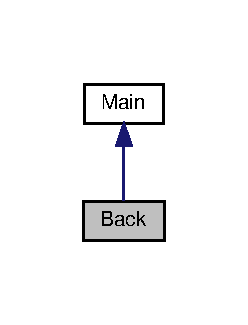
\includegraphics[width=119pt]{class_src_1_1_controllers_1_1_back__inherit__graph}
\end{center}
\end{figure}


Collaboration diagram for Back\+:
\nopagebreak
\begin{figure}[H]
\begin{center}
\leavevmode
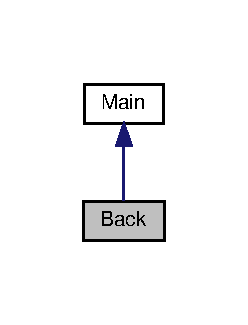
\includegraphics[width=119pt]{class_src_1_1_controllers_1_1_back__coll__graph}
\end{center}
\end{figure}
\subsection*{Public Member Functions}
\begin{DoxyCompactItemize}
\item 
\hyperlink{class_src_1_1_controllers_1_1_back_ac36db983080e1b0934908febca5de2d9}{Index} ()
\item 
\hyperlink{class_src_1_1_controllers_1_1_back_a405a66825259e2e811a2011a61c2beff}{Dashboard} ()
\item 
\hyperlink{class_src_1_1_controllers_1_1_back_a17e6c90f14225bdac5c65ed915b0a2f6}{List} ()
\item 
\hyperlink{class_src_1_1_controllers_1_1_back_abfd4f6736a8cd4dc4fa1e012996f4a23}{List\+Users} ()
\item 
\hyperlink{class_src_1_1_controllers_1_1_back_a384a1ec9e22b88a73de48023bb2bbf4f}{Check} (\$id)
\end{DoxyCompactItemize}
\subsection*{Additional Inherited Members}


\subsection{Detailed Description}
Classe \hyperlink{class_src_1_1_controllers_1_1_back}{Back} controleur pour les méthodes du back office si connecté en admin Hérite de la classe \hyperlink{class_src_1_1_controllers_1_1_main}{Main} 

\subsection{Member Function Documentation}
\mbox{\Hypertarget{class_src_1_1_controllers_1_1_back_a384a1ec9e22b88a73de48023bb2bbf4f}\label{class_src_1_1_controllers_1_1_back_a384a1ec9e22b88a73de48023bb2bbf4f}} 
\index{Src\+::\+Controllers\+::\+Back@{Src\+::\+Controllers\+::\+Back}!Check@{Check}}
\index{Check@{Check}!Src\+::\+Controllers\+::\+Back@{Src\+::\+Controllers\+::\+Back}}
\subsubsection{\texorpdfstring{Check()}{Check()}}
{\footnotesize\ttfamily Check (\begin{DoxyParamCaption}\item[{}]{\$id }\end{DoxyParamCaption})}

Vérification si commentaire est modéré 
\begin{DoxyParams}{Parameters}
{\em \$id} & suivant l\textquotesingle{}identifiant du commentaire . \\
\hline
\end{DoxyParams}
\mbox{\Hypertarget{class_src_1_1_controllers_1_1_back_a405a66825259e2e811a2011a61c2beff}\label{class_src_1_1_controllers_1_1_back_a405a66825259e2e811a2011a61c2beff}} 
\index{Src\+::\+Controllers\+::\+Back@{Src\+::\+Controllers\+::\+Back}!Dashboard@{Dashboard}}
\index{Dashboard@{Dashboard}!Src\+::\+Controllers\+::\+Back@{Src\+::\+Controllers\+::\+Back}}
\subsubsection{\texorpdfstring{Dashboard()}{Dashboard()}}
{\footnotesize\ttfamily Dashboard (\begin{DoxyParamCaption}{ }\end{DoxyParamCaption})}

Affichage Tableau de bord si connecté \mbox{\Hypertarget{class_src_1_1_controllers_1_1_back_ac36db983080e1b0934908febca5de2d9}\label{class_src_1_1_controllers_1_1_back_ac36db983080e1b0934908febca5de2d9}} 
\index{Src\+::\+Controllers\+::\+Back@{Src\+::\+Controllers\+::\+Back}!Index@{Index}}
\index{Index@{Index}!Src\+::\+Controllers\+::\+Back@{Src\+::\+Controllers\+::\+Back}}
\subsubsection{\texorpdfstring{Index()}{Index()}}
{\footnotesize\ttfamily Index (\begin{DoxyParamCaption}{ }\end{DoxyParamCaption})}

retour à l\textquotesingle{}accueil si déconnecté \mbox{\Hypertarget{class_src_1_1_controllers_1_1_back_a17e6c90f14225bdac5c65ed915b0a2f6}\label{class_src_1_1_controllers_1_1_back_a17e6c90f14225bdac5c65ed915b0a2f6}} 
\index{Src\+::\+Controllers\+::\+Back@{Src\+::\+Controllers\+::\+Back}!List@{List}}
\index{List@{List}!Src\+::\+Controllers\+::\+Back@{Src\+::\+Controllers\+::\+Back}}
\subsubsection{\texorpdfstring{List()}{List()}}
{\footnotesize\ttfamily List (\begin{DoxyParamCaption}{ }\end{DoxyParamCaption})}

Affichage de la liste des billets \mbox{\Hypertarget{class_src_1_1_controllers_1_1_back_abfd4f6736a8cd4dc4fa1e012996f4a23}\label{class_src_1_1_controllers_1_1_back_abfd4f6736a8cd4dc4fa1e012996f4a23}} 
\index{Src\+::\+Controllers\+::\+Back@{Src\+::\+Controllers\+::\+Back}!List\+Users@{List\+Users}}
\index{List\+Users@{List\+Users}!Src\+::\+Controllers\+::\+Back@{Src\+::\+Controllers\+::\+Back}}
\subsubsection{\texorpdfstring{List\+Users()}{ListUsers()}}
{\footnotesize\ttfamily List\+Users (\begin{DoxyParamCaption}{ }\end{DoxyParamCaption})}

Affichage de la liste des utilisateurs 

The documentation for this class was generated from the following file\+:\begin{DoxyCompactItemize}
\item 
Src/\+Controllers/\hyperlink{_back_8php}{Back.\+php}\end{DoxyCompactItemize}

\hypertarget{class_src_1_1_controllers_1_1_backedit}{}\section{Référence de la classe Backedit}
\label{class_src_1_1_controllers_1_1_backedit}\index{Backedit@{Backedit}}


Graphe d\textquotesingle{}héritage de Backedit\+:\nopagebreak
\begin{figure}[H]
\begin{center}
\leavevmode
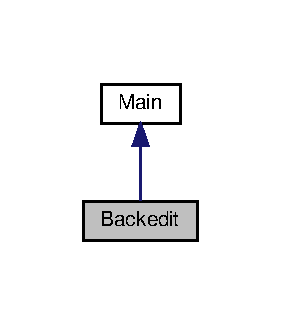
\includegraphics[width=135pt]{d2/d90/class_src_1_1_controllers_1_1_backedit__inherit__graph}
\end{center}
\end{figure}


Graphe de collaboration de Backedit\+:\nopagebreak
\begin{figure}[H]
\begin{center}
\leavevmode
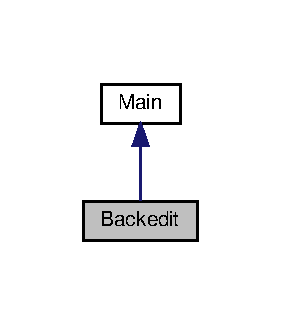
\includegraphics[width=135pt]{d0/dbb/class_src_1_1_controllers_1_1_backedit__coll__graph}
\end{center}
\end{figure}
\subsection*{Fonctions membres publiques}
\begin{DoxyCompactItemize}
\item 
\hyperlink{class_src_1_1_controllers_1_1_backedit_ad01f71fa0ecc039494e3c282864298c3}{Create} ()
\item 
\hyperlink{class_src_1_1_controllers_1_1_backedit_a82232b33fbfacdbdb8a8f49acaecf564}{Update} (\$id)
\item 
\hyperlink{class_src_1_1_controllers_1_1_backedit_af3369c06390987c5f54b6bc444c615ee}{Create\+\_\+user} ()
\item 
\hyperlink{class_src_1_1_controllers_1_1_backedit_ac76a9db7f422d94f155c99c21540da0e}{Update\+\_\+user} (\$id)
\item 
\hyperlink{class_src_1_1_controllers_1_1_backedit_a59113b5ecd1d155db6a4f30af34a1e80}{Delete} (\$id)
\item 
\hyperlink{class_src_1_1_controllers_1_1_backedit_a38147e014898a3417c74b23e903621b0}{Delete\+\_\+com} (\$id)
\item 
\hyperlink{class_src_1_1_controllers_1_1_backedit_ac8f9af14ff73b939d55940eb2ff886ee}{Delete\+\_\+user} (\$id)
\end{DoxyCompactItemize}
\subsection*{Membres hérités additionnels}


\subsection{Description détaillée}
Classe \hyperlink{class_src_1_1_controllers_1_1_backedit}{Backedit} gere la gestion des controleurs pour la modification des billets et commentaires si connecté Hérite de la calsse \hyperlink{class_src_1_1_controllers_1_1_main}{Main} 

Définition à la ligne 17 du fichier Backedit.\+php.



\subsection{Documentation des fonctions membres}
\mbox{\Hypertarget{class_src_1_1_controllers_1_1_backedit_ad01f71fa0ecc039494e3c282864298c3}\label{class_src_1_1_controllers_1_1_backedit_ad01f71fa0ecc039494e3c282864298c3}} 
\index{Src\+::\+Controllers\+::\+Backedit@{Src\+::\+Controllers\+::\+Backedit}!Create@{Create}}
\index{Create@{Create}!Src\+::\+Controllers\+::\+Backedit@{Src\+::\+Controllers\+::\+Backedit}}
\subsubsection{\texorpdfstring{Create()}{Create()}}
{\footnotesize\ttfamily Create (\begin{DoxyParamCaption}{ }\end{DoxyParamCaption})}

création d\textquotesingle{}un Billet 

Définition à la ligne 22 du fichier Backedit.\+php.

\mbox{\Hypertarget{class_src_1_1_controllers_1_1_backedit_af3369c06390987c5f54b6bc444c615ee}\label{class_src_1_1_controllers_1_1_backedit_af3369c06390987c5f54b6bc444c615ee}} 
\index{Src\+::\+Controllers\+::\+Backedit@{Src\+::\+Controllers\+::\+Backedit}!Create\+\_\+user@{Create\+\_\+user}}
\index{Create\+\_\+user@{Create\+\_\+user}!Src\+::\+Controllers\+::\+Backedit@{Src\+::\+Controllers\+::\+Backedit}}
\subsubsection{\texorpdfstring{Create\+\_\+user()}{Create\_user()}}
{\footnotesize\ttfamily Create\+\_\+user (\begin{DoxyParamCaption}{ }\end{DoxyParamCaption})}

Création d\textquotesingle{}un utilisateur 

Définition à la ligne 63 du fichier Backedit.\+php.

\mbox{\Hypertarget{class_src_1_1_controllers_1_1_backedit_a59113b5ecd1d155db6a4f30af34a1e80}\label{class_src_1_1_controllers_1_1_backedit_a59113b5ecd1d155db6a4f30af34a1e80}} 
\index{Src\+::\+Controllers\+::\+Backedit@{Src\+::\+Controllers\+::\+Backedit}!Delete@{Delete}}
\index{Delete@{Delete}!Src\+::\+Controllers\+::\+Backedit@{Src\+::\+Controllers\+::\+Backedit}}
\subsubsection{\texorpdfstring{Delete()}{Delete()}}
{\footnotesize\ttfamily Delete (\begin{DoxyParamCaption}\item[{}]{\$id }\end{DoxyParamCaption})}

Suppression d\textquotesingle{}un billet 
\begin{DoxyParams}[1]{Paramètres}
variable & {\em \$id} & identifiant du billet \\
\hline
\end{DoxyParams}


Définition à la ligne 106 du fichier Backedit.\+php.

\mbox{\Hypertarget{class_src_1_1_controllers_1_1_backedit_a38147e014898a3417c74b23e903621b0}\label{class_src_1_1_controllers_1_1_backedit_a38147e014898a3417c74b23e903621b0}} 
\index{Src\+::\+Controllers\+::\+Backedit@{Src\+::\+Controllers\+::\+Backedit}!Delete\+\_\+com@{Delete\+\_\+com}}
\index{Delete\+\_\+com@{Delete\+\_\+com}!Src\+::\+Controllers\+::\+Backedit@{Src\+::\+Controllers\+::\+Backedit}}
\subsubsection{\texorpdfstring{Delete\+\_\+com()}{Delete\_com()}}
{\footnotesize\ttfamily Delete\+\_\+com (\begin{DoxyParamCaption}\item[{}]{\$id }\end{DoxyParamCaption})}

Suppression d\textquotesingle{}un commentaire 
\begin{DoxyParams}[1]{Paramètres}
variable & {\em \$id} & identifiant du commentaire \\
\hline
\end{DoxyParams}


Définition à la ligne 121 du fichier Backedit.\+php.

\mbox{\Hypertarget{class_src_1_1_controllers_1_1_backedit_ac8f9af14ff73b939d55940eb2ff886ee}\label{class_src_1_1_controllers_1_1_backedit_ac8f9af14ff73b939d55940eb2ff886ee}} 
\index{Src\+::\+Controllers\+::\+Backedit@{Src\+::\+Controllers\+::\+Backedit}!Delete\+\_\+user@{Delete\+\_\+user}}
\index{Delete\+\_\+user@{Delete\+\_\+user}!Src\+::\+Controllers\+::\+Backedit@{Src\+::\+Controllers\+::\+Backedit}}
\subsubsection{\texorpdfstring{Delete\+\_\+user()}{Delete\_user()}}
{\footnotesize\ttfamily Delete\+\_\+user (\begin{DoxyParamCaption}\item[{}]{\$id }\end{DoxyParamCaption})}

Suppression d\textquotesingle{}un utilisateur 
\begin{DoxyParams}[1]{Paramètres}
variable & {\em \$id} & identifiant de l\textquotesingle{}utilisateur \\
\hline
\end{DoxyParams}


Définition à la ligne 134 du fichier Backedit.\+php.

\mbox{\Hypertarget{class_src_1_1_controllers_1_1_backedit_a82232b33fbfacdbdb8a8f49acaecf564}\label{class_src_1_1_controllers_1_1_backedit_a82232b33fbfacdbdb8a8f49acaecf564}} 
\index{Src\+::\+Controllers\+::\+Backedit@{Src\+::\+Controllers\+::\+Backedit}!Update@{Update}}
\index{Update@{Update}!Src\+::\+Controllers\+::\+Backedit@{Src\+::\+Controllers\+::\+Backedit}}
\subsubsection{\texorpdfstring{Update()}{Update()}}
{\footnotesize\ttfamily Update (\begin{DoxyParamCaption}\item[{}]{\$id }\end{DoxyParamCaption})}

Mise à jour du billet 
\begin{DoxyParams}[1]{Paramètres}
variable & {\em \$id} & identifiant du billet \\
\hline
\end{DoxyParams}


Définition à la ligne 42 du fichier Backedit.\+php.

\mbox{\Hypertarget{class_src_1_1_controllers_1_1_backedit_ac76a9db7f422d94f155c99c21540da0e}\label{class_src_1_1_controllers_1_1_backedit_ac76a9db7f422d94f155c99c21540da0e}} 
\index{Src\+::\+Controllers\+::\+Backedit@{Src\+::\+Controllers\+::\+Backedit}!Update\+\_\+user@{Update\+\_\+user}}
\index{Update\+\_\+user@{Update\+\_\+user}!Src\+::\+Controllers\+::\+Backedit@{Src\+::\+Controllers\+::\+Backedit}}
\subsubsection{\texorpdfstring{Update\+\_\+user()}{Update\_user()}}
{\footnotesize\ttfamily Update\+\_\+user (\begin{DoxyParamCaption}\item[{}]{\$id }\end{DoxyParamCaption})}

Mise à jour d\textquotesingle{}un utilisateur  $\ast$
\begin{DoxyParams}[1]{Paramètres}
variable & {\em \$id} & identifiant de l\textquotesingle{}utilisateur \\
\hline
\end{DoxyParams}


Définition à la ligne 82 du fichier Backedit.\+php.



La documentation de cette classe a été générée à partir du fichier suivant \+:\begin{DoxyCompactItemize}
\item 
/var/www/html/\+Alaska/\+Src/\+Controllers/\hyperlink{_backedit_8php}{Backedit.\+php}\end{DoxyCompactItemize}

\hypertarget{class_src_1_1_entity_1_1_billet}{}\section{Billet Class Reference}
\label{class_src_1_1_entity_1_1_billet}\index{Billet@{Billet}}
\subsection*{Public Member Functions}
\begin{DoxyCompactItemize}
\item 
\hyperlink{class_src_1_1_entity_1_1_billet_ab3129f1d71e9f51353de9d551ea381d7}{\+\_\+\+\_\+construct} (\$data=\mbox{[}$\,$\mbox{]})
\item 
\hyperlink{class_src_1_1_entity_1_1_billet_afde85a369fc83b442db3cf5c6ac31d4a}{set\+Author} (\$author)
\item 
\hyperlink{class_src_1_1_entity_1_1_billet_a884ba9bb0d54bde7839e798db7964476}{set\+Title} (\$title)
\item 
\hyperlink{class_src_1_1_entity_1_1_billet_a04a5eddb7c3abc7bf31fa25b58f046bf}{set\+Content} (\$content)
\item 
\hyperlink{class_src_1_1_entity_1_1_billet_af785d0fb8da1ba24ec74c2f9f7e27c0a}{set\+Image} (\$image)
\item 
\hyperlink{class_src_1_1_entity_1_1_billet_ad12db04fd7abd82e8172ebee19c45ff1}{set\+Create\+\_\+at} (Date\+Time \$create\+\_\+at)
\item 
\hyperlink{class_src_1_1_entity_1_1_billet_a9f9f5983de6ae197176a80f55f113a6c}{set\+Modif\+\_\+at} (Date\+Time \$modif\+\_\+at)
\item 
\hyperlink{class_src_1_1_entity_1_1_billet_acee4aedcde0f95ac298a1a0ce86be082}{set\+Posted} (\$posted)
\item 
\hyperlink{class_src_1_1_entity_1_1_billet_a12251d0c022e9e21c137a105ff683f13}{get\+Id} ()
\item 
\hyperlink{class_src_1_1_entity_1_1_billet_a5286e30390ae3e1b274940286493dd24}{get\+Author} ()
\item 
\hyperlink{class_src_1_1_entity_1_1_billet_a95e859a4588a39a1824b717378a84c29}{get\+Title} ()
\item 
\hyperlink{class_src_1_1_entity_1_1_billet_a58e43f09a06ce4e29b192c4e17ce7915}{get\+Content} ()
\item 
\hyperlink{class_src_1_1_entity_1_1_billet_a2af8add37797384585cae101fb8cbfe7}{get\+Image} ()
\item 
\hyperlink{class_src_1_1_entity_1_1_billet_ae5e6c0bedcef3f514100c20ee92c901a}{get\+Create\+\_\+at} ()
\item 
\hyperlink{class_src_1_1_entity_1_1_billet_a5858386cc69be9863ed37e0ceb2697b1}{get\+Modif\+\_\+at} ()
\item 
\hyperlink{class_src_1_1_entity_1_1_billet_a4a91b6f2e5d3d9220ccbed241e1d2eb0}{get\+Posted} ()
\end{DoxyCompactItemize}


\subsection{Constructor \& Destructor Documentation}
\mbox{\Hypertarget{class_src_1_1_entity_1_1_billet_ab3129f1d71e9f51353de9d551ea381d7}\label{class_src_1_1_entity_1_1_billet_ab3129f1d71e9f51353de9d551ea381d7}} 
\index{Src\+::\+Entity\+::\+Billet@{Src\+::\+Entity\+::\+Billet}!\+\_\+\+\_\+construct@{\+\_\+\+\_\+construct}}
\index{\+\_\+\+\_\+construct@{\+\_\+\+\_\+construct}!Src\+::\+Entity\+::\+Billet@{Src\+::\+Entity\+::\+Billet}}
\subsubsection{\texorpdfstring{\+\_\+\+\_\+construct()}{\_\_construct()}}
{\footnotesize\ttfamily \+\_\+\+\_\+construct (\begin{DoxyParamCaption}\item[{}]{\$data = {\ttfamily \mbox{[}\mbox{]}} }\end{DoxyParamCaption})}

Initialisation des données vers l\textquotesingle{}hydratation 
\begin{DoxyParams}[1]{Parameters}
variable & {\em \$data} & qui est un tableau des données \\
\hline
\end{DoxyParams}


\subsection{Member Function Documentation}
\mbox{\Hypertarget{class_src_1_1_entity_1_1_billet_a5286e30390ae3e1b274940286493dd24}\label{class_src_1_1_entity_1_1_billet_a5286e30390ae3e1b274940286493dd24}} 
\index{Src\+::\+Entity\+::\+Billet@{Src\+::\+Entity\+::\+Billet}!get\+Author@{get\+Author}}
\index{get\+Author@{get\+Author}!Src\+::\+Entity\+::\+Billet@{Src\+::\+Entity\+::\+Billet}}
\subsubsection{\texorpdfstring{get\+Author()}{getAuthor()}}
{\footnotesize\ttfamily get\+Author (\begin{DoxyParamCaption}{ }\end{DoxyParamCaption})}

\mbox{\Hypertarget{class_src_1_1_entity_1_1_billet_a58e43f09a06ce4e29b192c4e17ce7915}\label{class_src_1_1_entity_1_1_billet_a58e43f09a06ce4e29b192c4e17ce7915}} 
\index{Src\+::\+Entity\+::\+Billet@{Src\+::\+Entity\+::\+Billet}!get\+Content@{get\+Content}}
\index{get\+Content@{get\+Content}!Src\+::\+Entity\+::\+Billet@{Src\+::\+Entity\+::\+Billet}}
\subsubsection{\texorpdfstring{get\+Content()}{getContent()}}
{\footnotesize\ttfamily get\+Content (\begin{DoxyParamCaption}{ }\end{DoxyParamCaption})}

\mbox{\Hypertarget{class_src_1_1_entity_1_1_billet_ae5e6c0bedcef3f514100c20ee92c901a}\label{class_src_1_1_entity_1_1_billet_ae5e6c0bedcef3f514100c20ee92c901a}} 
\index{Src\+::\+Entity\+::\+Billet@{Src\+::\+Entity\+::\+Billet}!get\+Create\+\_\+at@{get\+Create\+\_\+at}}
\index{get\+Create\+\_\+at@{get\+Create\+\_\+at}!Src\+::\+Entity\+::\+Billet@{Src\+::\+Entity\+::\+Billet}}
\subsubsection{\texorpdfstring{get\+Create\+\_\+at()}{getCreate\_at()}}
{\footnotesize\ttfamily get\+Create\+\_\+at (\begin{DoxyParamCaption}{ }\end{DoxyParamCaption})}

\mbox{\Hypertarget{class_src_1_1_entity_1_1_billet_a12251d0c022e9e21c137a105ff683f13}\label{class_src_1_1_entity_1_1_billet_a12251d0c022e9e21c137a105ff683f13}} 
\index{Src\+::\+Entity\+::\+Billet@{Src\+::\+Entity\+::\+Billet}!get\+Id@{get\+Id}}
\index{get\+Id@{get\+Id}!Src\+::\+Entity\+::\+Billet@{Src\+::\+Entity\+::\+Billet}}
\subsubsection{\texorpdfstring{get\+Id()}{getId()}}
{\footnotesize\ttfamily get\+Id (\begin{DoxyParamCaption}{ }\end{DoxyParamCaption})}

Mise en place des G\+E\+T\+T\+E\+RS \mbox{\Hypertarget{class_src_1_1_entity_1_1_billet_a2af8add37797384585cae101fb8cbfe7}\label{class_src_1_1_entity_1_1_billet_a2af8add37797384585cae101fb8cbfe7}} 
\index{Src\+::\+Entity\+::\+Billet@{Src\+::\+Entity\+::\+Billet}!get\+Image@{get\+Image}}
\index{get\+Image@{get\+Image}!Src\+::\+Entity\+::\+Billet@{Src\+::\+Entity\+::\+Billet}}
\subsubsection{\texorpdfstring{get\+Image()}{getImage()}}
{\footnotesize\ttfamily get\+Image (\begin{DoxyParamCaption}{ }\end{DoxyParamCaption})}

\mbox{\Hypertarget{class_src_1_1_entity_1_1_billet_a5858386cc69be9863ed37e0ceb2697b1}\label{class_src_1_1_entity_1_1_billet_a5858386cc69be9863ed37e0ceb2697b1}} 
\index{Src\+::\+Entity\+::\+Billet@{Src\+::\+Entity\+::\+Billet}!get\+Modif\+\_\+at@{get\+Modif\+\_\+at}}
\index{get\+Modif\+\_\+at@{get\+Modif\+\_\+at}!Src\+::\+Entity\+::\+Billet@{Src\+::\+Entity\+::\+Billet}}
\subsubsection{\texorpdfstring{get\+Modif\+\_\+at()}{getModif\_at()}}
{\footnotesize\ttfamily get\+Modif\+\_\+at (\begin{DoxyParamCaption}{ }\end{DoxyParamCaption})}

\mbox{\Hypertarget{class_src_1_1_entity_1_1_billet_a4a91b6f2e5d3d9220ccbed241e1d2eb0}\label{class_src_1_1_entity_1_1_billet_a4a91b6f2e5d3d9220ccbed241e1d2eb0}} 
\index{Src\+::\+Entity\+::\+Billet@{Src\+::\+Entity\+::\+Billet}!get\+Posted@{get\+Posted}}
\index{get\+Posted@{get\+Posted}!Src\+::\+Entity\+::\+Billet@{Src\+::\+Entity\+::\+Billet}}
\subsubsection{\texorpdfstring{get\+Posted()}{getPosted()}}
{\footnotesize\ttfamily get\+Posted (\begin{DoxyParamCaption}{ }\end{DoxyParamCaption})}

\mbox{\Hypertarget{class_src_1_1_entity_1_1_billet_a95e859a4588a39a1824b717378a84c29}\label{class_src_1_1_entity_1_1_billet_a95e859a4588a39a1824b717378a84c29}} 
\index{Src\+::\+Entity\+::\+Billet@{Src\+::\+Entity\+::\+Billet}!get\+Title@{get\+Title}}
\index{get\+Title@{get\+Title}!Src\+::\+Entity\+::\+Billet@{Src\+::\+Entity\+::\+Billet}}
\subsubsection{\texorpdfstring{get\+Title()}{getTitle()}}
{\footnotesize\ttfamily get\+Title (\begin{DoxyParamCaption}{ }\end{DoxyParamCaption})}

\mbox{\Hypertarget{class_src_1_1_entity_1_1_billet_afde85a369fc83b442db3cf5c6ac31d4a}\label{class_src_1_1_entity_1_1_billet_afde85a369fc83b442db3cf5c6ac31d4a}} 
\index{Src\+::\+Entity\+::\+Billet@{Src\+::\+Entity\+::\+Billet}!set\+Author@{set\+Author}}
\index{set\+Author@{set\+Author}!Src\+::\+Entity\+::\+Billet@{Src\+::\+Entity\+::\+Billet}}
\subsubsection{\texorpdfstring{set\+Author()}{setAuthor()}}
{\footnotesize\ttfamily set\+Author (\begin{DoxyParamCaption}\item[{}]{\$author }\end{DoxyParamCaption})}

Mise en place des Setters avec vérification de format \mbox{\Hypertarget{class_src_1_1_entity_1_1_billet_a04a5eddb7c3abc7bf31fa25b58f046bf}\label{class_src_1_1_entity_1_1_billet_a04a5eddb7c3abc7bf31fa25b58f046bf}} 
\index{Src\+::\+Entity\+::\+Billet@{Src\+::\+Entity\+::\+Billet}!set\+Content@{set\+Content}}
\index{set\+Content@{set\+Content}!Src\+::\+Entity\+::\+Billet@{Src\+::\+Entity\+::\+Billet}}
\subsubsection{\texorpdfstring{set\+Content()}{setContent()}}
{\footnotesize\ttfamily set\+Content (\begin{DoxyParamCaption}\item[{}]{\$content }\end{DoxyParamCaption})}

\mbox{\Hypertarget{class_src_1_1_entity_1_1_billet_ad12db04fd7abd82e8172ebee19c45ff1}\label{class_src_1_1_entity_1_1_billet_ad12db04fd7abd82e8172ebee19c45ff1}} 
\index{Src\+::\+Entity\+::\+Billet@{Src\+::\+Entity\+::\+Billet}!set\+Create\+\_\+at@{set\+Create\+\_\+at}}
\index{set\+Create\+\_\+at@{set\+Create\+\_\+at}!Src\+::\+Entity\+::\+Billet@{Src\+::\+Entity\+::\+Billet}}
\subsubsection{\texorpdfstring{set\+Create\+\_\+at()}{setCreate\_at()}}
{\footnotesize\ttfamily set\+Create\+\_\+at (\begin{DoxyParamCaption}\item[{Date\+Time}]{\$create\+\_\+at }\end{DoxyParamCaption})}

\mbox{\Hypertarget{class_src_1_1_entity_1_1_billet_af785d0fb8da1ba24ec74c2f9f7e27c0a}\label{class_src_1_1_entity_1_1_billet_af785d0fb8da1ba24ec74c2f9f7e27c0a}} 
\index{Src\+::\+Entity\+::\+Billet@{Src\+::\+Entity\+::\+Billet}!set\+Image@{set\+Image}}
\index{set\+Image@{set\+Image}!Src\+::\+Entity\+::\+Billet@{Src\+::\+Entity\+::\+Billet}}
\subsubsection{\texorpdfstring{set\+Image()}{setImage()}}
{\footnotesize\ttfamily set\+Image (\begin{DoxyParamCaption}\item[{}]{\$image }\end{DoxyParamCaption})}

\mbox{\Hypertarget{class_src_1_1_entity_1_1_billet_a9f9f5983de6ae197176a80f55f113a6c}\label{class_src_1_1_entity_1_1_billet_a9f9f5983de6ae197176a80f55f113a6c}} 
\index{Src\+::\+Entity\+::\+Billet@{Src\+::\+Entity\+::\+Billet}!set\+Modif\+\_\+at@{set\+Modif\+\_\+at}}
\index{set\+Modif\+\_\+at@{set\+Modif\+\_\+at}!Src\+::\+Entity\+::\+Billet@{Src\+::\+Entity\+::\+Billet}}
\subsubsection{\texorpdfstring{set\+Modif\+\_\+at()}{setModif\_at()}}
{\footnotesize\ttfamily set\+Modif\+\_\+at (\begin{DoxyParamCaption}\item[{Date\+Time}]{\$modif\+\_\+at }\end{DoxyParamCaption})}

\mbox{\Hypertarget{class_src_1_1_entity_1_1_billet_acee4aedcde0f95ac298a1a0ce86be082}\label{class_src_1_1_entity_1_1_billet_acee4aedcde0f95ac298a1a0ce86be082}} 
\index{Src\+::\+Entity\+::\+Billet@{Src\+::\+Entity\+::\+Billet}!set\+Posted@{set\+Posted}}
\index{set\+Posted@{set\+Posted}!Src\+::\+Entity\+::\+Billet@{Src\+::\+Entity\+::\+Billet}}
\subsubsection{\texorpdfstring{set\+Posted()}{setPosted()}}
{\footnotesize\ttfamily set\+Posted (\begin{DoxyParamCaption}\item[{}]{\$posted }\end{DoxyParamCaption})}

\mbox{\Hypertarget{class_src_1_1_entity_1_1_billet_a884ba9bb0d54bde7839e798db7964476}\label{class_src_1_1_entity_1_1_billet_a884ba9bb0d54bde7839e798db7964476}} 
\index{Src\+::\+Entity\+::\+Billet@{Src\+::\+Entity\+::\+Billet}!set\+Title@{set\+Title}}
\index{set\+Title@{set\+Title}!Src\+::\+Entity\+::\+Billet@{Src\+::\+Entity\+::\+Billet}}
\subsubsection{\texorpdfstring{set\+Title()}{setTitle()}}
{\footnotesize\ttfamily set\+Title (\begin{DoxyParamCaption}\item[{}]{\$title }\end{DoxyParamCaption})}



The documentation for this class was generated from the following file\+:\begin{DoxyCompactItemize}
\item 
Src/\+Entity/\hyperlink{_billet_8php}{Billet.\+php}\end{DoxyCompactItemize}

\hypertarget{class_src_1_1_managers_1_1billet_manager}{}\section{Référence de la classe billet\+Manager}
\label{class_src_1_1_managers_1_1billet_manager}\index{billet\+Manager@{billet\+Manager}}
\subsection*{Fonctions membres publiques}
\begin{DoxyCompactItemize}
\item 
\hyperlink{class_src_1_1_managers_1_1billet_manager_a095c5d389db211932136b53f25f39685}{\+\_\+\+\_\+construct} ()
\item 
\hyperlink{class_src_1_1_managers_1_1billet_manager_a24f9f6fa83eb8694eab0a87b2e6ad0b1}{Read\+All} ()
\item 
\hyperlink{class_src_1_1_managers_1_1billet_manager_af7e26a4a8ffd767a1265151f87860ddb}{Read\+Front} (\$offset, \$limit)
\item 
\hyperlink{class_src_1_1_managers_1_1billet_manager_ad2bbc9b3130abdfe3a9fc9e9fe36716f}{Read} (\$id)
\item 
\hyperlink{class_src_1_1_managers_1_1billet_manager_ad01f71fa0ecc039494e3c282864298c3}{Create} ()
\item 
\hyperlink{class_src_1_1_managers_1_1billet_manager_a82232b33fbfacdbdb8a8f49acaecf564}{Update} (\$id)
\item 
\hyperlink{class_src_1_1_managers_1_1billet_manager_a59113b5ecd1d155db6a4f30af34a1e80}{Delete} (\$id)
\end{DoxyCompactItemize}
\subsection*{Attributs protégés}
\begin{DoxyCompactItemize}
\item 
\hyperlink{class_src_1_1_managers_1_1billet_manager_a1e6d977917b70dce7e26cebad8438bf4}{\$\+\_\+pdo}
\end{DoxyCompactItemize}


\subsection{Description détaillée}
Class Manager des billets qui regroupe l\textquotesingle{}ensemble des fonctions concernant la gestion des billets 
\begin{DoxyParams}[1]{Paramètres}
variable & {\em \$\+\_\+pdo} & nouvelle instance de la classe Dbd base de données \\
\hline
\end{DoxyParams}


Définition à la ligne 18 du fichier billet\+Manager.\+php.



\subsection{Documentation des constructeurs et destructeur}
\mbox{\Hypertarget{class_src_1_1_managers_1_1billet_manager_a095c5d389db211932136b53f25f39685}\label{class_src_1_1_managers_1_1billet_manager_a095c5d389db211932136b53f25f39685}} 
\index{Src\+::\+Managers\+::billet\+Manager@{Src\+::\+Managers\+::billet\+Manager}!\+\_\+\+\_\+construct@{\+\_\+\+\_\+construct}}
\index{\+\_\+\+\_\+construct@{\+\_\+\+\_\+construct}!Src\+::\+Managers\+::billet\+Manager@{Src\+::\+Managers\+::billet\+Manager}}
\subsubsection{\texorpdfstring{\+\_\+\+\_\+construct()}{\_\_construct()}}
{\footnotesize\ttfamily \+\_\+\+\_\+construct (\begin{DoxyParamCaption}{ }\end{DoxyParamCaption})}



Définition à la ligne 22 du fichier billet\+Manager.\+php.



\subsection{Documentation des fonctions membres}
\mbox{\Hypertarget{class_src_1_1_managers_1_1billet_manager_ad01f71fa0ecc039494e3c282864298c3}\label{class_src_1_1_managers_1_1billet_manager_ad01f71fa0ecc039494e3c282864298c3}} 
\index{Src\+::\+Managers\+::billet\+Manager@{Src\+::\+Managers\+::billet\+Manager}!Create@{Create}}
\index{Create@{Create}!Src\+::\+Managers\+::billet\+Manager@{Src\+::\+Managers\+::billet\+Manager}}
\subsubsection{\texorpdfstring{Create()}{Create()}}
{\footnotesize\ttfamily Create (\begin{DoxyParamCaption}{ }\end{DoxyParamCaption})}

Création ou insertion dans la base de données du billet 

Définition à la ligne 70 du fichier billet\+Manager.\+php.

\mbox{\Hypertarget{class_src_1_1_managers_1_1billet_manager_a59113b5ecd1d155db6a4f30af34a1e80}\label{class_src_1_1_managers_1_1billet_manager_a59113b5ecd1d155db6a4f30af34a1e80}} 
\index{Src\+::\+Managers\+::billet\+Manager@{Src\+::\+Managers\+::billet\+Manager}!Delete@{Delete}}
\index{Delete@{Delete}!Src\+::\+Managers\+::billet\+Manager@{Src\+::\+Managers\+::billet\+Manager}}
\subsubsection{\texorpdfstring{Delete()}{Delete()}}
{\footnotesize\ttfamily Delete (\begin{DoxyParamCaption}\item[{}]{\$id }\end{DoxyParamCaption})}

Effacement d\textquotesingle{}un enregistrement suivant son identifiant 
\begin{DoxyParams}[1]{Paramètres}
variable & {\em \$id} & identifiant du billet \\
\hline
\end{DoxyParams}


Définition à la ligne 190 du fichier billet\+Manager.\+php.

\mbox{\Hypertarget{class_src_1_1_managers_1_1billet_manager_ad2bbc9b3130abdfe3a9fc9e9fe36716f}\label{class_src_1_1_managers_1_1billet_manager_ad2bbc9b3130abdfe3a9fc9e9fe36716f}} 
\index{Src\+::\+Managers\+::billet\+Manager@{Src\+::\+Managers\+::billet\+Manager}!Read@{Read}}
\index{Read@{Read}!Src\+::\+Managers\+::billet\+Manager@{Src\+::\+Managers\+::billet\+Manager}}
\subsubsection{\texorpdfstring{Read()}{Read()}}
{\footnotesize\ttfamily Read (\begin{DoxyParamCaption}\item[{}]{\$id }\end{DoxyParamCaption})}

Lecture d\textquotesingle{}un billet en fonction de l\textquotesingle{}identifiant 
\begin{DoxyParams}[1]{Paramètres}
variable & {\em \$id} & identifiant du billet à afficher \\
\hline
\end{DoxyParams}


Définition à la ligne 58 du fichier billet\+Manager.\+php.

\mbox{\Hypertarget{class_src_1_1_managers_1_1billet_manager_a24f9f6fa83eb8694eab0a87b2e6ad0b1}\label{class_src_1_1_managers_1_1billet_manager_a24f9f6fa83eb8694eab0a87b2e6ad0b1}} 
\index{Src\+::\+Managers\+::billet\+Manager@{Src\+::\+Managers\+::billet\+Manager}!Read\+All@{Read\+All}}
\index{Read\+All@{Read\+All}!Src\+::\+Managers\+::billet\+Manager@{Src\+::\+Managers\+::billet\+Manager}}
\subsubsection{\texorpdfstring{Read\+All()}{ReadAll()}}
{\footnotesize\ttfamily Read\+All (\begin{DoxyParamCaption}{ }\end{DoxyParamCaption})}

Fonction pour lire tous les billets si connecté en admin 

Définition à la ligne 29 du fichier billet\+Manager.\+php.

\mbox{\Hypertarget{class_src_1_1_managers_1_1billet_manager_af7e26a4a8ffd767a1265151f87860ddb}\label{class_src_1_1_managers_1_1billet_manager_af7e26a4a8ffd767a1265151f87860ddb}} 
\index{Src\+::\+Managers\+::billet\+Manager@{Src\+::\+Managers\+::billet\+Manager}!Read\+Front@{Read\+Front}}
\index{Read\+Front@{Read\+Front}!Src\+::\+Managers\+::billet\+Manager@{Src\+::\+Managers\+::billet\+Manager}}
\subsubsection{\texorpdfstring{Read\+Front()}{ReadFront()}}
{\footnotesize\ttfamily Read\+Front (\begin{DoxyParamCaption}\item[{}]{\$offset,  }\item[{}]{\$limit }\end{DoxyParamCaption})}

Lecture des billets pour la partie front du site 
\begin{DoxyParams}[1]{Paramètres}
variable & {\em \$offset} & détermine la position de départ dans la base de donnée \\
\hline
variable & {\em \$limit} & détermine le nombre de billet à afficher \\
\hline
\end{DoxyParams}


Définition à la ligne 44 du fichier billet\+Manager.\+php.

\mbox{\Hypertarget{class_src_1_1_managers_1_1billet_manager_a82232b33fbfacdbdb8a8f49acaecf564}\label{class_src_1_1_managers_1_1billet_manager_a82232b33fbfacdbdb8a8f49acaecf564}} 
\index{Src\+::\+Managers\+::billet\+Manager@{Src\+::\+Managers\+::billet\+Manager}!Update@{Update}}
\index{Update@{Update}!Src\+::\+Managers\+::billet\+Manager@{Src\+::\+Managers\+::billet\+Manager}}
\subsubsection{\texorpdfstring{Update()}{Update()}}
{\footnotesize\ttfamily Update (\begin{DoxyParamCaption}\item[{}]{\$id }\end{DoxyParamCaption})}

Mise a jour des infos du billet suivant son identifiant en base de données 
\begin{DoxyParams}[1]{Paramètres}
variable & {\em \$id} & identifiant du billet \\
\hline
\end{DoxyParams}


Définition à la ligne 135 du fichier billet\+Manager.\+php.



\subsection{Documentation des champs}
\mbox{\Hypertarget{class_src_1_1_managers_1_1billet_manager_a1e6d977917b70dce7e26cebad8438bf4}\label{class_src_1_1_managers_1_1billet_manager_a1e6d977917b70dce7e26cebad8438bf4}} 
\index{Src\+::\+Managers\+::billet\+Manager@{Src\+::\+Managers\+::billet\+Manager}!\$\+\_\+pdo@{\$\+\_\+pdo}}
\index{\$\+\_\+pdo@{\$\+\_\+pdo}!Src\+::\+Managers\+::billet\+Manager@{Src\+::\+Managers\+::billet\+Manager}}
\subsubsection{\texorpdfstring{\$\+\_\+pdo}{$\_pdo}}
{\footnotesize\ttfamily \$\+\_\+pdo\hspace{0.3cm}{\ttfamily [protected]}}



Définition à la ligne 20 du fichier billet\+Manager.\+php.



La documentation de cette classe a été générée à partir du fichier suivant \+:\begin{DoxyCompactItemize}
\item 
/var/www/html/\+Alaska/\+Src/\+Managers/\hyperlink{billet_manager_8php}{billet\+Manager.\+php}\end{DoxyCompactItemize}

\hypertarget{class_app_1_1_check}{}\section{Check Class Reference}
\label{class_app_1_1_check}\index{Check@{Check}}
\subsection*{Static Public Member Functions}
\begin{DoxyCompactItemize}
\item 
static \hyperlink{class_app_1_1_check_a762802022c6341f5a11a5bd2d24e374a}{verif\+Session} ()
\item 
static \hyperlink{class_app_1_1_check_a336fdbb25ca75f575c65d04924058db9}{mix\+Mdp} (\$pass)
\end{DoxyCompactItemize}


\subsection{Detailed Description}
Classe \hyperlink{class_app_1_1_check}{Check} pour verification de la session avec token de comparaison . 

\subsection{Member Function Documentation}
\mbox{\Hypertarget{class_app_1_1_check_a336fdbb25ca75f575c65d04924058db9}\label{class_app_1_1_check_a336fdbb25ca75f575c65d04924058db9}} 
\index{App\+::\+Check@{App\+::\+Check}!mix\+Mdp@{mix\+Mdp}}
\index{mix\+Mdp@{mix\+Mdp}!App\+::\+Check@{App\+::\+Check}}
\subsubsection{\texorpdfstring{mix\+Mdp()}{mixMdp()}}
{\footnotesize\ttfamily static mix\+Mdp (\begin{DoxyParamCaption}\item[{}]{\$pass }\end{DoxyParamCaption})\hspace{0.3cm}{\ttfamily [static]}}

Fonction de cryptage 
\begin{DoxyParams}[1]{Parameters}
variable & {\em \$pass} & egal au password. \\
\hline
\end{DoxyParams}
\mbox{\Hypertarget{class_app_1_1_check_a762802022c6341f5a11a5bd2d24e374a}\label{class_app_1_1_check_a762802022c6341f5a11a5bd2d24e374a}} 
\index{App\+::\+Check@{App\+::\+Check}!verif\+Session@{verif\+Session}}
\index{verif\+Session@{verif\+Session}!App\+::\+Check@{App\+::\+Check}}
\subsubsection{\texorpdfstring{verif\+Session()}{verifSession()}}
{\footnotesize\ttfamily static verif\+Session (\begin{DoxyParamCaption}{ }\end{DoxyParamCaption})\hspace{0.3cm}{\ttfamily [static]}}



The documentation for this class was generated from the following file\+:\begin{DoxyCompactItemize}
\item 
App/\hyperlink{_check_8php}{Check.\+php}\end{DoxyCompactItemize}

\hypertarget{class_src_1_1_entity_1_1_comment}{}\section{Référence de la classe Comment}
\label{class_src_1_1_entity_1_1_comment}\index{Comment@{Comment}}
\subsection*{Fonctions membres publiques}
\begin{DoxyCompactItemize}
\item 
\hyperlink{class_src_1_1_entity_1_1_comment_a594620c0e8c7693172eee4901c0b7705}{\+\_\+\+\_\+construct} (\$date=\mbox{[}$\,$\mbox{]})
\item 
\hyperlink{class_src_1_1_entity_1_1_comment_a1d65ce1d25ffb871a48d33715e6b6bef}{set\+Pseudo} (\$pseudo)
\item 
\hyperlink{class_src_1_1_entity_1_1_comment_a04a5eddb7c3abc7bf31fa25b58f046bf}{set\+Content} (\$content)
\item 
\hyperlink{class_src_1_1_entity_1_1_comment_ad12db04fd7abd82e8172ebee19c45ff1}{set\+Create\+\_\+at} (Date\+Time \$create\+\_\+at)
\item 
\hyperlink{class_src_1_1_entity_1_1_comment_a9f9f5983de6ae197176a80f55f113a6c}{set\+Modif\+\_\+at} (Date\+Time \$modif\+\_\+at)
\item 
\hyperlink{class_src_1_1_entity_1_1_comment_a2e409e601842718df8e3fb392a6553a2}{set\+Bil\+\_\+\+Id} (\$bil\+\_\+id)
\item 
\hyperlink{class_src_1_1_entity_1_1_comment_a0067c44a7d1de40089ffed311672b328}{set\+Moderate} (\$moderate)
\item 
\hyperlink{class_src_1_1_entity_1_1_comment_a12251d0c022e9e21c137a105ff683f13}{get\+Id} ()
\item 
\hyperlink{class_src_1_1_entity_1_1_comment_a7151e41f7b522d26d02102d970e9a309}{get\+Pseudo} ()
\item 
\hyperlink{class_src_1_1_entity_1_1_comment_a58e43f09a06ce4e29b192c4e17ce7915}{get\+Content} ()
\item 
\hyperlink{class_src_1_1_entity_1_1_comment_ae5e6c0bedcef3f514100c20ee92c901a}{get\+Create\+\_\+at} ()
\item 
\hyperlink{class_src_1_1_entity_1_1_comment_a5858386cc69be9863ed37e0ceb2697b1}{get\+Modif\+\_\+at} ()
\item 
\hyperlink{class_src_1_1_entity_1_1_comment_a1df6ee009c81d0d807d36d18d40b9e97}{get\+Bil\+\_\+id} ()
\item 
\hyperlink{class_src_1_1_entity_1_1_comment_a6d3a6a148bf0c8752548e7e7ab149abb}{get\+Moderate} ()
\end{DoxyCompactItemize}


\subsection{Description détaillée}


Définition à la ligne 15 du fichier Comment.\+php.



\subsection{Documentation des constructeurs et destructeur}
\mbox{\Hypertarget{class_src_1_1_entity_1_1_comment_a594620c0e8c7693172eee4901c0b7705}\label{class_src_1_1_entity_1_1_comment_a594620c0e8c7693172eee4901c0b7705}} 
\index{Src\+::\+Entity\+::\+Comment@{Src\+::\+Entity\+::\+Comment}!\+\_\+\+\_\+construct@{\+\_\+\+\_\+construct}}
\index{\+\_\+\+\_\+construct@{\+\_\+\+\_\+construct}!Src\+::\+Entity\+::\+Comment@{Src\+::\+Entity\+::\+Comment}}
\subsubsection{\texorpdfstring{\+\_\+\+\_\+construct()}{\_\_construct()}}
{\footnotesize\ttfamily \+\_\+\+\_\+construct (\begin{DoxyParamCaption}\item[{}]{\$date = {\ttfamily \mbox{[}\mbox{]}} }\end{DoxyParamCaption})}

Initialisation des données vers l\textquotesingle{}hydratation 
\begin{DoxyParams}[1]{Paramètres}
variable & {\em \$data} & qui est un tableau des données \\
\hline
\end{DoxyParams}


Définition à la ligne 28 du fichier Comment.\+php.



\subsection{Documentation des fonctions membres}
\mbox{\Hypertarget{class_src_1_1_entity_1_1_comment_a1df6ee009c81d0d807d36d18d40b9e97}\label{class_src_1_1_entity_1_1_comment_a1df6ee009c81d0d807d36d18d40b9e97}} 
\index{Src\+::\+Entity\+::\+Comment@{Src\+::\+Entity\+::\+Comment}!get\+Bil\+\_\+id@{get\+Bil\+\_\+id}}
\index{get\+Bil\+\_\+id@{get\+Bil\+\_\+id}!Src\+::\+Entity\+::\+Comment@{Src\+::\+Entity\+::\+Comment}}
\subsubsection{\texorpdfstring{get\+Bil\+\_\+id()}{getBil\_id()}}
{\footnotesize\ttfamily get\+Bil\+\_\+id (\begin{DoxyParamCaption}{ }\end{DoxyParamCaption})}



Définition à la ligne 98 du fichier Comment.\+php.

\mbox{\Hypertarget{class_src_1_1_entity_1_1_comment_a58e43f09a06ce4e29b192c4e17ce7915}\label{class_src_1_1_entity_1_1_comment_a58e43f09a06ce4e29b192c4e17ce7915}} 
\index{Src\+::\+Entity\+::\+Comment@{Src\+::\+Entity\+::\+Comment}!get\+Content@{get\+Content}}
\index{get\+Content@{get\+Content}!Src\+::\+Entity\+::\+Comment@{Src\+::\+Entity\+::\+Comment}}
\subsubsection{\texorpdfstring{get\+Content()}{getContent()}}
{\footnotesize\ttfamily get\+Content (\begin{DoxyParamCaption}{ }\end{DoxyParamCaption})}



Définition à la ligne 86 du fichier Comment.\+php.

\mbox{\Hypertarget{class_src_1_1_entity_1_1_comment_ae5e6c0bedcef3f514100c20ee92c901a}\label{class_src_1_1_entity_1_1_comment_ae5e6c0bedcef3f514100c20ee92c901a}} 
\index{Src\+::\+Entity\+::\+Comment@{Src\+::\+Entity\+::\+Comment}!get\+Create\+\_\+at@{get\+Create\+\_\+at}}
\index{get\+Create\+\_\+at@{get\+Create\+\_\+at}!Src\+::\+Entity\+::\+Comment@{Src\+::\+Entity\+::\+Comment}}
\subsubsection{\texorpdfstring{get\+Create\+\_\+at()}{getCreate\_at()}}
{\footnotesize\ttfamily get\+Create\+\_\+at (\begin{DoxyParamCaption}{ }\end{DoxyParamCaption})}



Définition à la ligne 90 du fichier Comment.\+php.

\mbox{\Hypertarget{class_src_1_1_entity_1_1_comment_a12251d0c022e9e21c137a105ff683f13}\label{class_src_1_1_entity_1_1_comment_a12251d0c022e9e21c137a105ff683f13}} 
\index{Src\+::\+Entity\+::\+Comment@{Src\+::\+Entity\+::\+Comment}!get\+Id@{get\+Id}}
\index{get\+Id@{get\+Id}!Src\+::\+Entity\+::\+Comment@{Src\+::\+Entity\+::\+Comment}}
\subsubsection{\texorpdfstring{get\+Id()}{getId()}}
{\footnotesize\ttfamily get\+Id (\begin{DoxyParamCaption}{ }\end{DoxyParamCaption})}

Mise en place des G\+E\+T\+T\+E\+RS 

Définition à la ligne 78 du fichier Comment.\+php.

\mbox{\Hypertarget{class_src_1_1_entity_1_1_comment_a6d3a6a148bf0c8752548e7e7ab149abb}\label{class_src_1_1_entity_1_1_comment_a6d3a6a148bf0c8752548e7e7ab149abb}} 
\index{Src\+::\+Entity\+::\+Comment@{Src\+::\+Entity\+::\+Comment}!get\+Moderate@{get\+Moderate}}
\index{get\+Moderate@{get\+Moderate}!Src\+::\+Entity\+::\+Comment@{Src\+::\+Entity\+::\+Comment}}
\subsubsection{\texorpdfstring{get\+Moderate()}{getModerate()}}
{\footnotesize\ttfamily get\+Moderate (\begin{DoxyParamCaption}{ }\end{DoxyParamCaption})}



Définition à la ligne 102 du fichier Comment.\+php.

\mbox{\Hypertarget{class_src_1_1_entity_1_1_comment_a5858386cc69be9863ed37e0ceb2697b1}\label{class_src_1_1_entity_1_1_comment_a5858386cc69be9863ed37e0ceb2697b1}} 
\index{Src\+::\+Entity\+::\+Comment@{Src\+::\+Entity\+::\+Comment}!get\+Modif\+\_\+at@{get\+Modif\+\_\+at}}
\index{get\+Modif\+\_\+at@{get\+Modif\+\_\+at}!Src\+::\+Entity\+::\+Comment@{Src\+::\+Entity\+::\+Comment}}
\subsubsection{\texorpdfstring{get\+Modif\+\_\+at()}{getModif\_at()}}
{\footnotesize\ttfamily get\+Modif\+\_\+at (\begin{DoxyParamCaption}{ }\end{DoxyParamCaption})}



Définition à la ligne 94 du fichier Comment.\+php.

\mbox{\Hypertarget{class_src_1_1_entity_1_1_comment_a7151e41f7b522d26d02102d970e9a309}\label{class_src_1_1_entity_1_1_comment_a7151e41f7b522d26d02102d970e9a309}} 
\index{Src\+::\+Entity\+::\+Comment@{Src\+::\+Entity\+::\+Comment}!get\+Pseudo@{get\+Pseudo}}
\index{get\+Pseudo@{get\+Pseudo}!Src\+::\+Entity\+::\+Comment@{Src\+::\+Entity\+::\+Comment}}
\subsubsection{\texorpdfstring{get\+Pseudo()}{getPseudo()}}
{\footnotesize\ttfamily get\+Pseudo (\begin{DoxyParamCaption}{ }\end{DoxyParamCaption})}



Définition à la ligne 82 du fichier Comment.\+php.

\mbox{\Hypertarget{class_src_1_1_entity_1_1_comment_a2e409e601842718df8e3fb392a6553a2}\label{class_src_1_1_entity_1_1_comment_a2e409e601842718df8e3fb392a6553a2}} 
\index{Src\+::\+Entity\+::\+Comment@{Src\+::\+Entity\+::\+Comment}!set\+Bil\+\_\+\+Id@{set\+Bil\+\_\+\+Id}}
\index{set\+Bil\+\_\+\+Id@{set\+Bil\+\_\+\+Id}!Src\+::\+Entity\+::\+Comment@{Src\+::\+Entity\+::\+Comment}}
\subsubsection{\texorpdfstring{set\+Bil\+\_\+\+Id()}{setBil\_Id()}}
{\footnotesize\ttfamily set\+Bil\+\_\+\+Id (\begin{DoxyParamCaption}\item[{}]{\$bil\+\_\+id }\end{DoxyParamCaption})}



Définition à la ligne 65 du fichier Comment.\+php.

\mbox{\Hypertarget{class_src_1_1_entity_1_1_comment_a04a5eddb7c3abc7bf31fa25b58f046bf}\label{class_src_1_1_entity_1_1_comment_a04a5eddb7c3abc7bf31fa25b58f046bf}} 
\index{Src\+::\+Entity\+::\+Comment@{Src\+::\+Entity\+::\+Comment}!set\+Content@{set\+Content}}
\index{set\+Content@{set\+Content}!Src\+::\+Entity\+::\+Comment@{Src\+::\+Entity\+::\+Comment}}
\subsubsection{\texorpdfstring{set\+Content()}{setContent()}}
{\footnotesize\ttfamily set\+Content (\begin{DoxyParamCaption}\item[{}]{\$content }\end{DoxyParamCaption})}



Définition à la ligne 49 du fichier Comment.\+php.

\mbox{\Hypertarget{class_src_1_1_entity_1_1_comment_ad12db04fd7abd82e8172ebee19c45ff1}\label{class_src_1_1_entity_1_1_comment_ad12db04fd7abd82e8172ebee19c45ff1}} 
\index{Src\+::\+Entity\+::\+Comment@{Src\+::\+Entity\+::\+Comment}!set\+Create\+\_\+at@{set\+Create\+\_\+at}}
\index{set\+Create\+\_\+at@{set\+Create\+\_\+at}!Src\+::\+Entity\+::\+Comment@{Src\+::\+Entity\+::\+Comment}}
\subsubsection{\texorpdfstring{set\+Create\+\_\+at()}{setCreate\_at()}}
{\footnotesize\ttfamily set\+Create\+\_\+at (\begin{DoxyParamCaption}\item[{Date\+Time}]{\$create\+\_\+at }\end{DoxyParamCaption})}



Définition à la ligne 57 du fichier Comment.\+php.

\mbox{\Hypertarget{class_src_1_1_entity_1_1_comment_a0067c44a7d1de40089ffed311672b328}\label{class_src_1_1_entity_1_1_comment_a0067c44a7d1de40089ffed311672b328}} 
\index{Src\+::\+Entity\+::\+Comment@{Src\+::\+Entity\+::\+Comment}!set\+Moderate@{set\+Moderate}}
\index{set\+Moderate@{set\+Moderate}!Src\+::\+Entity\+::\+Comment@{Src\+::\+Entity\+::\+Comment}}
\subsubsection{\texorpdfstring{set\+Moderate()}{setModerate()}}
{\footnotesize\ttfamily set\+Moderate (\begin{DoxyParamCaption}\item[{}]{\$moderate }\end{DoxyParamCaption})}



Définition à la ligne 69 du fichier Comment.\+php.

\mbox{\Hypertarget{class_src_1_1_entity_1_1_comment_a9f9f5983de6ae197176a80f55f113a6c}\label{class_src_1_1_entity_1_1_comment_a9f9f5983de6ae197176a80f55f113a6c}} 
\index{Src\+::\+Entity\+::\+Comment@{Src\+::\+Entity\+::\+Comment}!set\+Modif\+\_\+at@{set\+Modif\+\_\+at}}
\index{set\+Modif\+\_\+at@{set\+Modif\+\_\+at}!Src\+::\+Entity\+::\+Comment@{Src\+::\+Entity\+::\+Comment}}
\subsubsection{\texorpdfstring{set\+Modif\+\_\+at()}{setModif\_at()}}
{\footnotesize\ttfamily set\+Modif\+\_\+at (\begin{DoxyParamCaption}\item[{Date\+Time}]{\$modif\+\_\+at }\end{DoxyParamCaption})}



Définition à la ligne 61 du fichier Comment.\+php.

\mbox{\Hypertarget{class_src_1_1_entity_1_1_comment_a1d65ce1d25ffb871a48d33715e6b6bef}\label{class_src_1_1_entity_1_1_comment_a1d65ce1d25ffb871a48d33715e6b6bef}} 
\index{Src\+::\+Entity\+::\+Comment@{Src\+::\+Entity\+::\+Comment}!set\+Pseudo@{set\+Pseudo}}
\index{set\+Pseudo@{set\+Pseudo}!Src\+::\+Entity\+::\+Comment@{Src\+::\+Entity\+::\+Comment}}
\subsubsection{\texorpdfstring{set\+Pseudo()}{setPseudo()}}
{\footnotesize\ttfamily set\+Pseudo (\begin{DoxyParamCaption}\item[{}]{\$pseudo }\end{DoxyParamCaption})}

Mise en place des S\+E\+T\+T\+E\+RS avec vérification de format de données 

Définition à la ligne 41 du fichier Comment.\+php.



La documentation de cette classe a été générée à partir du fichier suivant \+:\begin{DoxyCompactItemize}
\item 
/var/www/html/\+Alaska/\+Src/\+Entity/\hyperlink{_comment_8php}{Comment.\+php}\end{DoxyCompactItemize}

\hypertarget{class_src_1_1_managers_1_1comment_manager}{}\section{Référence de la classe comment\+Manager}
\label{class_src_1_1_managers_1_1comment_manager}\index{comment\+Manager@{comment\+Manager}}
\subsection*{Fonctions membres publiques}
\begin{DoxyCompactItemize}
\item 
\hyperlink{class_src_1_1_managers_1_1comment_manager_a095c5d389db211932136b53f25f39685}{\+\_\+\+\_\+construct} ()
\item 
\hyperlink{class_src_1_1_managers_1_1comment_manager_a24f9f6fa83eb8694eab0a87b2e6ad0b1}{Read\+All} ()
\item 
\hyperlink{class_src_1_1_managers_1_1comment_manager_a4224d6d3de965c48624a2c530d0a2c94}{Read\+Moderate} ()
\item 
\hyperlink{class_src_1_1_managers_1_1comment_manager_af0b2d518844625de0b1fe21ebb8e6c58}{Read} (\$id=null)
\item 
\hyperlink{class_src_1_1_managers_1_1comment_manager_ad01f71fa0ecc039494e3c282864298c3}{Create} ()
\item 
\hyperlink{class_src_1_1_managers_1_1comment_manager_a511df177d885f133ac59c2b68c7046f2}{Moderate} (\$id)
\item 
\hyperlink{class_src_1_1_managers_1_1comment_manager_a59113b5ecd1d155db6a4f30af34a1e80}{Delete} (\$id)
\end{DoxyCompactItemize}
\subsection*{Attributs protégés}
\begin{DoxyCompactItemize}
\item 
\hyperlink{class_src_1_1_managers_1_1comment_manager_a1e6d977917b70dce7e26cebad8438bf4}{\$\+\_\+pdo}
\end{DoxyCompactItemize}


\subsection{Description détaillée}
Classe Manager des commentaires qui regroupes les fonctions pour la gestion des commentaires. 
\begin{DoxyParams}[1]{Paramètres}
variable & {\em \$\+\_\+pdo} & nouvelle instance de la classe Dbd base de données \\
\hline
\end{DoxyParams}


Définition à la ligne 19 du fichier comment\+Manager.\+php.



\subsection{Documentation des constructeurs et destructeur}
\mbox{\Hypertarget{class_src_1_1_managers_1_1comment_manager_a095c5d389db211932136b53f25f39685}\label{class_src_1_1_managers_1_1comment_manager_a095c5d389db211932136b53f25f39685}} 
\index{Src\+::\+Managers\+::comment\+Manager@{Src\+::\+Managers\+::comment\+Manager}!\+\_\+\+\_\+construct@{\+\_\+\+\_\+construct}}
\index{\+\_\+\+\_\+construct@{\+\_\+\+\_\+construct}!Src\+::\+Managers\+::comment\+Manager@{Src\+::\+Managers\+::comment\+Manager}}
\subsubsection{\texorpdfstring{\+\_\+\+\_\+construct()}{\_\_construct()}}
{\footnotesize\ttfamily \+\_\+\+\_\+construct (\begin{DoxyParamCaption}{ }\end{DoxyParamCaption})}



Définition à la ligne 23 du fichier comment\+Manager.\+php.



\subsection{Documentation des fonctions membres}
\mbox{\Hypertarget{class_src_1_1_managers_1_1comment_manager_ad01f71fa0ecc039494e3c282864298c3}\label{class_src_1_1_managers_1_1comment_manager_ad01f71fa0ecc039494e3c282864298c3}} 
\index{Src\+::\+Managers\+::comment\+Manager@{Src\+::\+Managers\+::comment\+Manager}!Create@{Create}}
\index{Create@{Create}!Src\+::\+Managers\+::comment\+Manager@{Src\+::\+Managers\+::comment\+Manager}}
\subsubsection{\texorpdfstring{Create()}{Create()}}
{\footnotesize\ttfamily Create (\begin{DoxyParamCaption}{ }\end{DoxyParamCaption})}

Fonction de création ou insertion de commentaire dans le base de données 

Définition à la ligne 75 du fichier comment\+Manager.\+php.

\mbox{\Hypertarget{class_src_1_1_managers_1_1comment_manager_a59113b5ecd1d155db6a4f30af34a1e80}\label{class_src_1_1_managers_1_1comment_manager_a59113b5ecd1d155db6a4f30af34a1e80}} 
\index{Src\+::\+Managers\+::comment\+Manager@{Src\+::\+Managers\+::comment\+Manager}!Delete@{Delete}}
\index{Delete@{Delete}!Src\+::\+Managers\+::comment\+Manager@{Src\+::\+Managers\+::comment\+Manager}}
\subsubsection{\texorpdfstring{Delete()}{Delete()}}
{\footnotesize\ttfamily Delete (\begin{DoxyParamCaption}\item[{}]{\$id }\end{DoxyParamCaption})}

Fonction d\textquotesingle{}effacement du commentaire 
\begin{DoxyParams}[1]{Paramètres}
variable & {\em \$id} & identifiant du commentaire \\
\hline
\end{DoxyParams}


Définition à la ligne 143 du fichier comment\+Manager.\+php.

\mbox{\Hypertarget{class_src_1_1_managers_1_1comment_manager_a511df177d885f133ac59c2b68c7046f2}\label{class_src_1_1_managers_1_1comment_manager_a511df177d885f133ac59c2b68c7046f2}} 
\index{Src\+::\+Managers\+::comment\+Manager@{Src\+::\+Managers\+::comment\+Manager}!Moderate@{Moderate}}
\index{Moderate@{Moderate}!Src\+::\+Managers\+::comment\+Manager@{Src\+::\+Managers\+::comment\+Manager}}
\subsubsection{\texorpdfstring{Moderate()}{Moderate()}}
{\footnotesize\ttfamily Moderate (\begin{DoxyParamCaption}\item[{}]{\$id }\end{DoxyParamCaption})}

Fonction de modération verification sur létat de \textquotesingle{}moderate\textquotesingle{} dans la base de données puis si l\textquotesingle{}etat est non signaler le passe en signaler et inversement 
\begin{DoxyParams}[1]{Paramètres}
variable & {\em \$id} & identifiant du commentaire \\
\hline
\end{DoxyParams}


Définition à la ligne 121 du fichier comment\+Manager.\+php.

\mbox{\Hypertarget{class_src_1_1_managers_1_1comment_manager_af0b2d518844625de0b1fe21ebb8e6c58}\label{class_src_1_1_managers_1_1comment_manager_af0b2d518844625de0b1fe21ebb8e6c58}} 
\index{Src\+::\+Managers\+::comment\+Manager@{Src\+::\+Managers\+::comment\+Manager}!Read@{Read}}
\index{Read@{Read}!Src\+::\+Managers\+::comment\+Manager@{Src\+::\+Managers\+::comment\+Manager}}
\subsubsection{\texorpdfstring{Read()}{Read()}}
{\footnotesize\ttfamily Read (\begin{DoxyParamCaption}\item[{}]{\$id = {\ttfamily null} }\end{DoxyParamCaption})}

Fonction de lecture d\textquotesingle{}un commentaire avec ou sans id 
\begin{DoxyParams}[1]{Paramètres}
variable & {\em \$id} & identifiant du commentaire \\
\hline
\end{DoxyParams}


Définition à la ligne 55 du fichier comment\+Manager.\+php.

\mbox{\Hypertarget{class_src_1_1_managers_1_1comment_manager_a24f9f6fa83eb8694eab0a87b2e6ad0b1}\label{class_src_1_1_managers_1_1comment_manager_a24f9f6fa83eb8694eab0a87b2e6ad0b1}} 
\index{Src\+::\+Managers\+::comment\+Manager@{Src\+::\+Managers\+::comment\+Manager}!Read\+All@{Read\+All}}
\index{Read\+All@{Read\+All}!Src\+::\+Managers\+::comment\+Manager@{Src\+::\+Managers\+::comment\+Manager}}
\subsubsection{\texorpdfstring{Read\+All()}{ReadAll()}}
{\footnotesize\ttfamily Read\+All (\begin{DoxyParamCaption}{ }\end{DoxyParamCaption})}

Fonction de lecture de tous ls commentaires 

Définition à la ligne 30 du fichier comment\+Manager.\+php.

\mbox{\Hypertarget{class_src_1_1_managers_1_1comment_manager_a4224d6d3de965c48624a2c530d0a2c94}\label{class_src_1_1_managers_1_1comment_manager_a4224d6d3de965c48624a2c530d0a2c94}} 
\index{Src\+::\+Managers\+::comment\+Manager@{Src\+::\+Managers\+::comment\+Manager}!Read\+Moderate@{Read\+Moderate}}
\index{Read\+Moderate@{Read\+Moderate}!Src\+::\+Managers\+::comment\+Manager@{Src\+::\+Managers\+::comment\+Manager}}
\subsubsection{\texorpdfstring{Read\+Moderate()}{ReadModerate()}}
{\footnotesize\ttfamily Read\+Moderate (\begin{DoxyParamCaption}{ }\end{DoxyParamCaption})}

Fonction de lecture des commentaires qui ont moderate = à 1 donc signaler pour l\textquotesingle{}admin 

Définition à la ligne 42 du fichier comment\+Manager.\+php.



\subsection{Documentation des champs}
\mbox{\Hypertarget{class_src_1_1_managers_1_1comment_manager_a1e6d977917b70dce7e26cebad8438bf4}\label{class_src_1_1_managers_1_1comment_manager_a1e6d977917b70dce7e26cebad8438bf4}} 
\index{Src\+::\+Managers\+::comment\+Manager@{Src\+::\+Managers\+::comment\+Manager}!\$\+\_\+pdo@{\$\+\_\+pdo}}
\index{\$\+\_\+pdo@{\$\+\_\+pdo}!Src\+::\+Managers\+::comment\+Manager@{Src\+::\+Managers\+::comment\+Manager}}
\subsubsection{\texorpdfstring{\$\+\_\+pdo}{$\_pdo}}
{\footnotesize\ttfamily \$\+\_\+pdo\hspace{0.3cm}{\ttfamily [protected]}}



Définition à la ligne 21 du fichier comment\+Manager.\+php.



La documentation de cette classe a été générée à partir du fichier suivant \+:\begin{DoxyCompactItemize}
\item 
/var/www/html/\+Alaska/\+Src/\+Managers/\hyperlink{comment_manager_8php}{comment\+Manager.\+php}\end{DoxyCompactItemize}

\hypertarget{class_app_1_1_dbd}{}\section{Dbd Class Reference}
\label{class_app_1_1_dbd}\index{Dbd@{Dbd}}


Inheritance diagram for Dbd\+:
\nopagebreak
\begin{figure}[H]
\begin{center}
\leavevmode
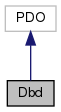
\includegraphics[width=118pt]{class_app_1_1_dbd__inherit__graph}
\end{center}
\end{figure}


Collaboration diagram for Dbd\+:
\nopagebreak
\begin{figure}[H]
\begin{center}
\leavevmode
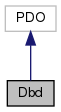
\includegraphics[width=118pt]{class_app_1_1_dbd__coll__graph}
\end{center}
\end{figure}
\subsection*{Public Member Functions}
\begin{DoxyCompactItemize}
\item 
\hyperlink{class_app_1_1_dbd_a095c5d389db211932136b53f25f39685}{\+\_\+\+\_\+construct} ()
\end{DoxyCompactItemize}


\subsection{Detailed Description}
Classe de connexion à la base de données Utilisation des constances de la classe config pour les parametres de connexion 

\subsection{Constructor \& Destructor Documentation}
\mbox{\Hypertarget{class_app_1_1_dbd_a095c5d389db211932136b53f25f39685}\label{class_app_1_1_dbd_a095c5d389db211932136b53f25f39685}} 
\index{App\+::\+Dbd@{App\+::\+Dbd}!\+\_\+\+\_\+construct@{\+\_\+\+\_\+construct}}
\index{\+\_\+\+\_\+construct@{\+\_\+\+\_\+construct}!App\+::\+Dbd@{App\+::\+Dbd}}
\subsubsection{\texorpdfstring{\+\_\+\+\_\+construct()}{\_\_construct()}}
{\footnotesize\ttfamily \+\_\+\+\_\+construct (\begin{DoxyParamCaption}{ }\end{DoxyParamCaption})}



The documentation for this class was generated from the following file\+:\begin{DoxyCompactItemize}
\item 
App/\hyperlink{_dbd_8php}{Dbd.\+php}\end{DoxyCompactItemize}

\section{Front Class Reference}
\label{class_src_1_1_controllers_1_1_front}\index{Front@{Front}}


Inheritance diagram for Front\+:
\nopagebreak
\begin{figure}[H]
\begin{center}
\leavevmode
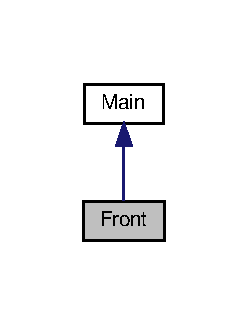
\includegraphics[width=119pt]{class_src_1_1_controllers_1_1_front__inherit__graph}
\end{center}
\end{figure}


Collaboration diagram for Front\+:
\nopagebreak
\begin{figure}[H]
\begin{center}
\leavevmode
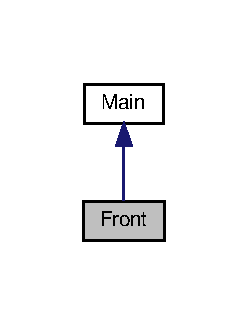
\includegraphics[width=119pt]{class_src_1_1_controllers_1_1_front__coll__graph}
\end{center}
\end{figure}
\subsection*{Public Member Functions}
\begin{DoxyCompactItemize}
\item 
\textbf{ Index} ()
\item 
\textbf{ Posting} (\$id)
\item 
\textbf{ List} ()
\item 
\textbf{ Create} ()
\item 
\textbf{ Signaler} (\$id)
\end{DoxyCompactItemize}
\subsection*{Data Fields}
\begin{DoxyCompactItemize}
\item 
const \textbf{ M\+A\+X\+\_\+\+P\+O\+ST} = 4
\end{DoxyCompactItemize}
\subsection*{Additional Inherited Members}


\subsection{Detailed Description}


Definition at line 6 of file Front.\+php.



\subsection{Member Function Documentation}
\mbox{\label{class_src_1_1_controllers_1_1_front_ad01f71fa0ecc039494e3c282864298c3}} 
\index{Src\+::\+Controllers\+::\+Front@{Src\+::\+Controllers\+::\+Front}!Create@{Create}}
\index{Create@{Create}!Src\+::\+Controllers\+::\+Front@{Src\+::\+Controllers\+::\+Front}}
\subsubsection{Create()}
{\footnotesize\ttfamily Create (\begin{DoxyParamCaption}{ }\end{DoxyParamCaption})}



Definition at line 33 of file Front.\+php.

\mbox{\label{class_src_1_1_controllers_1_1_front_ac36db983080e1b0934908febca5de2d9}} 
\index{Src\+::\+Controllers\+::\+Front@{Src\+::\+Controllers\+::\+Front}!Index@{Index}}
\index{Index@{Index}!Src\+::\+Controllers\+::\+Front@{Src\+::\+Controllers\+::\+Front}}
\subsubsection{Index()}
{\footnotesize\ttfamily Index (\begin{DoxyParamCaption}{ }\end{DoxyParamCaption})}



Definition at line 11 of file Front.\+php.

\mbox{\label{class_src_1_1_controllers_1_1_front_a17e6c90f14225bdac5c65ed915b0a2f6}} 
\index{Src\+::\+Controllers\+::\+Front@{Src\+::\+Controllers\+::\+Front}!List@{List}}
\index{List@{List}!Src\+::\+Controllers\+::\+Front@{Src\+::\+Controllers\+::\+Front}}
\subsubsection{List()}
{\footnotesize\ttfamily List (\begin{DoxyParamCaption}{ }\end{DoxyParamCaption})}



Definition at line 26 of file Front.\+php.

\mbox{\label{class_src_1_1_controllers_1_1_front_a5fcbe325afb03acc6e4eaec38a7bb1ae}} 
\index{Src\+::\+Controllers\+::\+Front@{Src\+::\+Controllers\+::\+Front}!Posting@{Posting}}
\index{Posting@{Posting}!Src\+::\+Controllers\+::\+Front@{Src\+::\+Controllers\+::\+Front}}
\subsubsection{Posting()}
{\footnotesize\ttfamily Posting (\begin{DoxyParamCaption}\item[{}]{\$id }\end{DoxyParamCaption})}



Definition at line 18 of file Front.\+php.

\mbox{\label{class_src_1_1_controllers_1_1_front_a8b22c40bd1737bbb7db0816b7e9763b3}} 
\index{Src\+::\+Controllers\+::\+Front@{Src\+::\+Controllers\+::\+Front}!Signaler@{Signaler}}
\index{Signaler@{Signaler}!Src\+::\+Controllers\+::\+Front@{Src\+::\+Controllers\+::\+Front}}
\subsubsection{Signaler()}
{\footnotesize\ttfamily Signaler (\begin{DoxyParamCaption}\item[{}]{\$id }\end{DoxyParamCaption})}



Definition at line 42 of file Front.\+php.



\subsection{Field Documentation}
\mbox{\label{class_src_1_1_controllers_1_1_front_ae6f0a6c86ad9f61cbc99ad3c4180b481}} 
\index{Src\+::\+Controllers\+::\+Front@{Src\+::\+Controllers\+::\+Front}!M\+A\+X\+\_\+\+P\+O\+ST@{M\+A\+X\+\_\+\+P\+O\+ST}}
\index{M\+A\+X\+\_\+\+P\+O\+ST@{M\+A\+X\+\_\+\+P\+O\+ST}!Src\+::\+Controllers\+::\+Front@{Src\+::\+Controllers\+::\+Front}}
\subsubsection{M\+A\+X\+\_\+\+P\+O\+ST}
{\footnotesize\ttfamily const M\+A\+X\+\_\+\+P\+O\+ST = 4}



Definition at line 8 of file Front.\+php.



The documentation for this class was generated from the following file\+:\begin{DoxyCompactItemize}
\item 
Src/\+Controllers/\textbf{ Front.\+php}\end{DoxyCompactItemize}

\hypertarget{class_src_1_1_controllers_1_1_main}{}\section{Référence de la classe Main}
\label{class_src_1_1_controllers_1_1_main}\index{Main@{Main}}


Graphe d\textquotesingle{}héritage de Main\+:\nopagebreak
\begin{figure}[H]
\begin{center}
\leavevmode
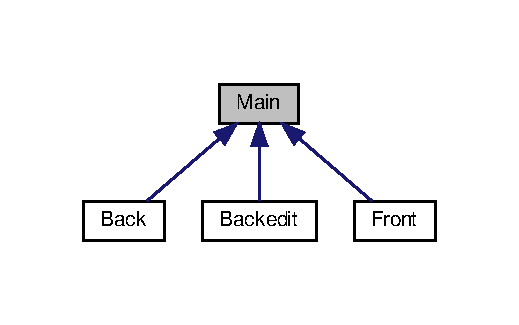
\includegraphics[width=249pt]{d9/dca/class_src_1_1_controllers_1_1_main__inherit__graph}
\end{center}
\end{figure}
\subsection*{Fonctions membres publiques}
\begin{DoxyCompactItemize}
\item 
\hyperlink{class_src_1_1_controllers_1_1_main_a095c5d389db211932136b53f25f39685}{\+\_\+\+\_\+construct} ()
\item 
\hyperlink{class_src_1_1_controllers_1_1_main_a8db48c2902872da0ee80463db6696375}{Login} ()
\item 
\hyperlink{class_src_1_1_controllers_1_1_main_aba348654bb87049dfb96fa24794b191b}{Signup} ()
\item 
\hyperlink{class_src_1_1_controllers_1_1_main_aa14f760d541a59acb41ac8eefddafb9b}{Logout} ()
\end{DoxyCompactItemize}
\subsection*{Attributs protégés}
\begin{DoxyCompactItemize}
\item 
\hyperlink{class_src_1_1_controllers_1_1_main_a7205c4d22c61e375f2be552a32f97ccb}{\$billet\+Manager}
\item 
\hyperlink{class_src_1_1_controllers_1_1_main_a2fdbb2dc79956746757958a453709ca6}{\$comment\+Manager}
\item 
\hyperlink{class_src_1_1_controllers_1_1_main_afd45ca85c50f41c20a03f0a8d0f4db23}{\$user\+Manager}
\end{DoxyCompactItemize}


\subsection{Description détaillée}
Class \hyperlink{class_src_1_1_controllers_1_1_main}{Main} instancie les classes controllers et vérifie la connection et l\textquotesingle{}inscription sur le site ainsi que la déconnexion. 
\begin{DoxyParams}{Paramètres}
{\em \$\+\_\+id} & = l\textquotesingle{}identifiant des Entities. \\
\hline
{\em \$billet\+Manager} & = instance de la classse Billet Manager \\
\hline
{\em \$comment\+Manager} & = instance de la classe Comment Manager \\
\hline
{\em \$user\+Manager} & = instance de la calsse User Manager \\
\hline
\end{DoxyParams}


Définition à la ligne 23 du fichier Main.\+php.



\subsection{Documentation des constructeurs et destructeur}
\mbox{\Hypertarget{class_src_1_1_controllers_1_1_main_a095c5d389db211932136b53f25f39685}\label{class_src_1_1_controllers_1_1_main_a095c5d389db211932136b53f25f39685}} 
\index{Src\+::\+Controllers\+::\+Main@{Src\+::\+Controllers\+::\+Main}!\+\_\+\+\_\+construct@{\+\_\+\+\_\+construct}}
\index{\+\_\+\+\_\+construct@{\+\_\+\+\_\+construct}!Src\+::\+Controllers\+::\+Main@{Src\+::\+Controllers\+::\+Main}}
\subsubsection{\texorpdfstring{\+\_\+\+\_\+construct()}{\_\_construct()}}
{\footnotesize\ttfamily \+\_\+\+\_\+construct (\begin{DoxyParamCaption}{ }\end{DoxyParamCaption})}

Instanceiation des classes et de la session et mise verification de l\textquotesingle{}identifiant 

Définition à la ligne 33 du fichier Main.\+php.



\subsection{Documentation des fonctions membres}
\mbox{\Hypertarget{class_src_1_1_controllers_1_1_main_a8db48c2902872da0ee80463db6696375}\label{class_src_1_1_controllers_1_1_main_a8db48c2902872da0ee80463db6696375}} 
\index{Src\+::\+Controllers\+::\+Main@{Src\+::\+Controllers\+::\+Main}!Login@{Login}}
\index{Login@{Login}!Src\+::\+Controllers\+::\+Main@{Src\+::\+Controllers\+::\+Main}}
\subsubsection{\texorpdfstring{Login()}{Login()}}
{\footnotesize\ttfamily Login (\begin{DoxyParamCaption}{ }\end{DoxyParamCaption})}

Page de connexion a la partie Admin 

Définition à la ligne 47 du fichier Main.\+php.

\mbox{\Hypertarget{class_src_1_1_controllers_1_1_main_aa14f760d541a59acb41ac8eefddafb9b}\label{class_src_1_1_controllers_1_1_main_aa14f760d541a59acb41ac8eefddafb9b}} 
\index{Src\+::\+Controllers\+::\+Main@{Src\+::\+Controllers\+::\+Main}!Logout@{Logout}}
\index{Logout@{Logout}!Src\+::\+Controllers\+::\+Main@{Src\+::\+Controllers\+::\+Main}}
\subsubsection{\texorpdfstring{Logout()}{Logout()}}
{\footnotesize\ttfamily Logout (\begin{DoxyParamCaption}{ }\end{DoxyParamCaption})}

Déconnection de la partie Admin 

Définition à la ligne 78 du fichier Main.\+php.

\mbox{\Hypertarget{class_src_1_1_controllers_1_1_main_aba348654bb87049dfb96fa24794b191b}\label{class_src_1_1_controllers_1_1_main_aba348654bb87049dfb96fa24794b191b}} 
\index{Src\+::\+Controllers\+::\+Main@{Src\+::\+Controllers\+::\+Main}!Signup@{Signup}}
\index{Signup@{Signup}!Src\+::\+Controllers\+::\+Main@{Src\+::\+Controllers\+::\+Main}}
\subsubsection{\texorpdfstring{Signup()}{Signup()}}
{\footnotesize\ttfamily Signup (\begin{DoxyParamCaption}{ }\end{DoxyParamCaption})}

Inscription utilisateur 

Définition à la ligne 62 du fichier Main.\+php.



\subsection{Documentation des champs}
\mbox{\Hypertarget{class_src_1_1_controllers_1_1_main_a7205c4d22c61e375f2be552a32f97ccb}\label{class_src_1_1_controllers_1_1_main_a7205c4d22c61e375f2be552a32f97ccb}} 
\index{Src\+::\+Controllers\+::\+Main@{Src\+::\+Controllers\+::\+Main}!\$billet\+Manager@{\$billet\+Manager}}
\index{\$billet\+Manager@{\$billet\+Manager}!Src\+::\+Controllers\+::\+Main@{Src\+::\+Controllers\+::\+Main}}
\subsubsection{\texorpdfstring{\$billet\+Manager}{$billetManager}}
{\footnotesize\ttfamily \$\hyperlink{class_src_1_1_managers_1_1billet_manager}{billet\+Manager}\hspace{0.3cm}{\ttfamily [protected]}}



Définition à la ligne 26 du fichier Main.\+php.

\mbox{\Hypertarget{class_src_1_1_controllers_1_1_main_a2fdbb2dc79956746757958a453709ca6}\label{class_src_1_1_controllers_1_1_main_a2fdbb2dc79956746757958a453709ca6}} 
\index{Src\+::\+Controllers\+::\+Main@{Src\+::\+Controllers\+::\+Main}!\$comment\+Manager@{\$comment\+Manager}}
\index{\$comment\+Manager@{\$comment\+Manager}!Src\+::\+Controllers\+::\+Main@{Src\+::\+Controllers\+::\+Main}}
\subsubsection{\texorpdfstring{\$comment\+Manager}{$commentManager}}
{\footnotesize\ttfamily \$\hyperlink{class_src_1_1_managers_1_1comment_manager}{comment\+Manager}\hspace{0.3cm}{\ttfamily [protected]}}



Définition à la ligne 27 du fichier Main.\+php.

\mbox{\Hypertarget{class_src_1_1_controllers_1_1_main_afd45ca85c50f41c20a03f0a8d0f4db23}\label{class_src_1_1_controllers_1_1_main_afd45ca85c50f41c20a03f0a8d0f4db23}} 
\index{Src\+::\+Controllers\+::\+Main@{Src\+::\+Controllers\+::\+Main}!\$user\+Manager@{\$user\+Manager}}
\index{\$user\+Manager@{\$user\+Manager}!Src\+::\+Controllers\+::\+Main@{Src\+::\+Controllers\+::\+Main}}
\subsubsection{\texorpdfstring{\$user\+Manager}{$userManager}}
{\footnotesize\ttfamily \$\hyperlink{class_src_1_1_managers_1_1user_manager}{user\+Manager}\hspace{0.3cm}{\ttfamily [protected]}}



Définition à la ligne 28 du fichier Main.\+php.



La documentation de cette classe a été générée à partir du fichier suivant \+:\begin{DoxyCompactItemize}
\item 
/var/www/html/\+Alaska/\+Src/\+Controllers/\hyperlink{_main_8php}{Main.\+php}\end{DoxyCompactItemize}

\section{Router Class Reference}
\label{class_app_1_1_router}\index{Router@{Router}}
\subsection*{Public Member Functions}
\begin{DoxyCompactItemize}
\item 
\textbf{ \+\_\+\+\_\+construct} ()
\item 
\textbf{ init\+Route} ()
\end{DoxyCompactItemize}


\subsection{Detailed Description}


Definition at line 9 of file Router.\+php.



\subsection{Constructor \& Destructor Documentation}
\mbox{\label{class_app_1_1_router_a095c5d389db211932136b53f25f39685}} 
\index{App\+::\+Router@{App\+::\+Router}!\+\_\+\+\_\+construct@{\+\_\+\+\_\+construct}}
\index{\+\_\+\+\_\+construct@{\+\_\+\+\_\+construct}!App\+::\+Router@{App\+::\+Router}}
\subsubsection{\+\_\+\+\_\+construct()}
{\footnotesize\ttfamily \+\_\+\+\_\+construct (\begin{DoxyParamCaption}{ }\end{DoxyParamCaption})}



Definition at line 12 of file Router.\+php.



\subsection{Member Function Documentation}
\mbox{\label{class_app_1_1_router_a6fa8800727e8e7eeab56d569bfa3429b}} 
\index{App\+::\+Router@{App\+::\+Router}!init\+Route@{init\+Route}}
\index{init\+Route@{init\+Route}!App\+::\+Router@{App\+::\+Router}}
\subsubsection{init\+Route()}
{\footnotesize\ttfamily init\+Route (\begin{DoxyParamCaption}{ }\end{DoxyParamCaption})}



Definition at line 19 of file Router.\+php.



The documentation for this class was generated from the following file\+:\begin{DoxyCompactItemize}
\item 
App/\textbf{ Router.\+php}\end{DoxyCompactItemize}

\hypertarget{class_src_1_1_entity_1_1_user}{}\section{Référence de la classe User}
\label{class_src_1_1_entity_1_1_user}\index{User@{User}}
\subsection*{Fonctions membres publiques}
\begin{DoxyCompactItemize}
\item 
\hyperlink{class_src_1_1_entity_1_1_user_ab3129f1d71e9f51353de9d551ea381d7}{\+\_\+\+\_\+construct} (\$data=\mbox{[}$\,$\mbox{]})
\item 
\hyperlink{class_src_1_1_entity_1_1_user_ac359b701a2ccaff746dd480f03314244}{set\+Username} (\$username)
\item 
\hyperlink{class_src_1_1_entity_1_1_user_a5ef76eef42d2624386442eeb636d338c}{set\+Email} (\$email)
\item 
\hyperlink{class_src_1_1_entity_1_1_user_a3e35c8d3dbb2c513c618a664389e0926}{set\+Password} (\$password)
\item 
\hyperlink{class_src_1_1_entity_1_1_user_a9c8311c6d2e7d1d118a6a6da7b577c0b}{set\+Date\+Crea} (Date\+Time \$create\+\_\+at)
\item 
\hyperlink{class_src_1_1_entity_1_1_user_a9f9f5983de6ae197176a80f55f113a6c}{set\+Modif\+\_\+at} (Date\+Time \$modif\+\_\+at)
\item 
\hyperlink{class_src_1_1_entity_1_1_user_a12251d0c022e9e21c137a105ff683f13}{get\+Id} ()
\item 
\hyperlink{class_src_1_1_entity_1_1_user_a81b37a3c9d639574e394f80c1138c75e}{get\+Username} ()
\item 
\hyperlink{class_src_1_1_entity_1_1_user_a02a01849f28e2535e888ae4ec87b20f2}{get\+Email} ()
\item 
\hyperlink{class_src_1_1_entity_1_1_user_a04e0957baeb7acde9c0c86556da2d43f}{get\+Password} ()
\item 
\hyperlink{class_src_1_1_entity_1_1_user_ae5e6c0bedcef3f514100c20ee92c901a}{get\+Create\+\_\+at} ()
\item 
\hyperlink{class_src_1_1_entity_1_1_user_a5858386cc69be9863ed37e0ceb2697b1}{get\+Modif\+\_\+at} ()
\end{DoxyCompactItemize}


\subsection{Description détaillée}


Définition à la ligne 15 du fichier User.\+php.



\subsection{Documentation des constructeurs et destructeur}
\mbox{\Hypertarget{class_src_1_1_entity_1_1_user_ab3129f1d71e9f51353de9d551ea381d7}\label{class_src_1_1_entity_1_1_user_ab3129f1d71e9f51353de9d551ea381d7}} 
\index{Src\+::\+Entity\+::\+User@{Src\+::\+Entity\+::\+User}!\+\_\+\+\_\+construct@{\+\_\+\+\_\+construct}}
\index{\+\_\+\+\_\+construct@{\+\_\+\+\_\+construct}!Src\+::\+Entity\+::\+User@{Src\+::\+Entity\+::\+User}}
\subsubsection{\texorpdfstring{\+\_\+\+\_\+construct()}{\_\_construct()}}
{\footnotesize\ttfamily \+\_\+\+\_\+construct (\begin{DoxyParamCaption}\item[{}]{\$data = {\ttfamily \mbox{[}\mbox{]}} }\end{DoxyParamCaption})}

Initialisation des données vers l\textquotesingle{}hydratation 
\begin{DoxyParams}[1]{Paramètres}
variable & {\em \$data} & qui est un tableau des données \\
\hline
\end{DoxyParams}


Définition à la ligne 27 du fichier User.\+php.



\subsection{Documentation des fonctions membres}
\mbox{\Hypertarget{class_src_1_1_entity_1_1_user_ae5e6c0bedcef3f514100c20ee92c901a}\label{class_src_1_1_entity_1_1_user_ae5e6c0bedcef3f514100c20ee92c901a}} 
\index{Src\+::\+Entity\+::\+User@{Src\+::\+Entity\+::\+User}!get\+Create\+\_\+at@{get\+Create\+\_\+at}}
\index{get\+Create\+\_\+at@{get\+Create\+\_\+at}!Src\+::\+Entity\+::\+User@{Src\+::\+Entity\+::\+User}}
\subsubsection{\texorpdfstring{get\+Create\+\_\+at()}{getCreate\_at()}}
{\footnotesize\ttfamily get\+Create\+\_\+at (\begin{DoxyParamCaption}{ }\end{DoxyParamCaption})}



Définition à la ligne 95 du fichier User.\+php.

\mbox{\Hypertarget{class_src_1_1_entity_1_1_user_a02a01849f28e2535e888ae4ec87b20f2}\label{class_src_1_1_entity_1_1_user_a02a01849f28e2535e888ae4ec87b20f2}} 
\index{Src\+::\+Entity\+::\+User@{Src\+::\+Entity\+::\+User}!get\+Email@{get\+Email}}
\index{get\+Email@{get\+Email}!Src\+::\+Entity\+::\+User@{Src\+::\+Entity\+::\+User}}
\subsubsection{\texorpdfstring{get\+Email()}{getEmail()}}
{\footnotesize\ttfamily get\+Email (\begin{DoxyParamCaption}{ }\end{DoxyParamCaption})}



Définition à la ligne 87 du fichier User.\+php.

\mbox{\Hypertarget{class_src_1_1_entity_1_1_user_a12251d0c022e9e21c137a105ff683f13}\label{class_src_1_1_entity_1_1_user_a12251d0c022e9e21c137a105ff683f13}} 
\index{Src\+::\+Entity\+::\+User@{Src\+::\+Entity\+::\+User}!get\+Id@{get\+Id}}
\index{get\+Id@{get\+Id}!Src\+::\+Entity\+::\+User@{Src\+::\+Entity\+::\+User}}
\subsubsection{\texorpdfstring{get\+Id()}{getId()}}
{\footnotesize\ttfamily get\+Id (\begin{DoxyParamCaption}{ }\end{DoxyParamCaption})}

Mise en place des G\+E\+T\+T\+E\+RS 

Définition à la ligne 79 du fichier User.\+php.

\mbox{\Hypertarget{class_src_1_1_entity_1_1_user_a5858386cc69be9863ed37e0ceb2697b1}\label{class_src_1_1_entity_1_1_user_a5858386cc69be9863ed37e0ceb2697b1}} 
\index{Src\+::\+Entity\+::\+User@{Src\+::\+Entity\+::\+User}!get\+Modif\+\_\+at@{get\+Modif\+\_\+at}}
\index{get\+Modif\+\_\+at@{get\+Modif\+\_\+at}!Src\+::\+Entity\+::\+User@{Src\+::\+Entity\+::\+User}}
\subsubsection{\texorpdfstring{get\+Modif\+\_\+at()}{getModif\_at()}}
{\footnotesize\ttfamily get\+Modif\+\_\+at (\begin{DoxyParamCaption}{ }\end{DoxyParamCaption})}



Définition à la ligne 99 du fichier User.\+php.

\mbox{\Hypertarget{class_src_1_1_entity_1_1_user_a04e0957baeb7acde9c0c86556da2d43f}\label{class_src_1_1_entity_1_1_user_a04e0957baeb7acde9c0c86556da2d43f}} 
\index{Src\+::\+Entity\+::\+User@{Src\+::\+Entity\+::\+User}!get\+Password@{get\+Password}}
\index{get\+Password@{get\+Password}!Src\+::\+Entity\+::\+User@{Src\+::\+Entity\+::\+User}}
\subsubsection{\texorpdfstring{get\+Password()}{getPassword()}}
{\footnotesize\ttfamily get\+Password (\begin{DoxyParamCaption}{ }\end{DoxyParamCaption})}



Définition à la ligne 91 du fichier User.\+php.

\mbox{\Hypertarget{class_src_1_1_entity_1_1_user_a81b37a3c9d639574e394f80c1138c75e}\label{class_src_1_1_entity_1_1_user_a81b37a3c9d639574e394f80c1138c75e}} 
\index{Src\+::\+Entity\+::\+User@{Src\+::\+Entity\+::\+User}!get\+Username@{get\+Username}}
\index{get\+Username@{get\+Username}!Src\+::\+Entity\+::\+User@{Src\+::\+Entity\+::\+User}}
\subsubsection{\texorpdfstring{get\+Username()}{getUsername()}}
{\footnotesize\ttfamily get\+Username (\begin{DoxyParamCaption}{ }\end{DoxyParamCaption})}



Définition à la ligne 83 du fichier User.\+php.

\mbox{\Hypertarget{class_src_1_1_entity_1_1_user_a9c8311c6d2e7d1d118a6a6da7b577c0b}\label{class_src_1_1_entity_1_1_user_a9c8311c6d2e7d1d118a6a6da7b577c0b}} 
\index{Src\+::\+Entity\+::\+User@{Src\+::\+Entity\+::\+User}!set\+Date\+Crea@{set\+Date\+Crea}}
\index{set\+Date\+Crea@{set\+Date\+Crea}!Src\+::\+Entity\+::\+User@{Src\+::\+Entity\+::\+User}}
\subsubsection{\texorpdfstring{set\+Date\+Crea()}{setDateCrea()}}
{\footnotesize\ttfamily set\+Date\+Crea (\begin{DoxyParamCaption}\item[{Date\+Time}]{\$create\+\_\+at }\end{DoxyParamCaption})}



Définition à la ligne 64 du fichier User.\+php.

\mbox{\Hypertarget{class_src_1_1_entity_1_1_user_a5ef76eef42d2624386442eeb636d338c}\label{class_src_1_1_entity_1_1_user_a5ef76eef42d2624386442eeb636d338c}} 
\index{Src\+::\+Entity\+::\+User@{Src\+::\+Entity\+::\+User}!set\+Email@{set\+Email}}
\index{set\+Email@{set\+Email}!Src\+::\+Entity\+::\+User@{Src\+::\+Entity\+::\+User}}
\subsubsection{\texorpdfstring{set\+Email()}{setEmail()}}
{\footnotesize\ttfamily set\+Email (\begin{DoxyParamCaption}\item[{}]{\$email }\end{DoxyParamCaption})}



Définition à la ligne 48 du fichier User.\+php.

\mbox{\Hypertarget{class_src_1_1_entity_1_1_user_a9f9f5983de6ae197176a80f55f113a6c}\label{class_src_1_1_entity_1_1_user_a9f9f5983de6ae197176a80f55f113a6c}} 
\index{Src\+::\+Entity\+::\+User@{Src\+::\+Entity\+::\+User}!set\+Modif\+\_\+at@{set\+Modif\+\_\+at}}
\index{set\+Modif\+\_\+at@{set\+Modif\+\_\+at}!Src\+::\+Entity\+::\+User@{Src\+::\+Entity\+::\+User}}
\subsubsection{\texorpdfstring{set\+Modif\+\_\+at()}{setModif\_at()}}
{\footnotesize\ttfamily set\+Modif\+\_\+at (\begin{DoxyParamCaption}\item[{Date\+Time}]{\$modif\+\_\+at }\end{DoxyParamCaption})}



Définition à la ligne 70 du fichier User.\+php.

\mbox{\Hypertarget{class_src_1_1_entity_1_1_user_a3e35c8d3dbb2c513c618a664389e0926}\label{class_src_1_1_entity_1_1_user_a3e35c8d3dbb2c513c618a664389e0926}} 
\index{Src\+::\+Entity\+::\+User@{Src\+::\+Entity\+::\+User}!set\+Password@{set\+Password}}
\index{set\+Password@{set\+Password}!Src\+::\+Entity\+::\+User@{Src\+::\+Entity\+::\+User}}
\subsubsection{\texorpdfstring{set\+Password()}{setPassword()}}
{\footnotesize\ttfamily set\+Password (\begin{DoxyParamCaption}\item[{}]{\$password }\end{DoxyParamCaption})}



Définition à la ligne 56 du fichier User.\+php.

\mbox{\Hypertarget{class_src_1_1_entity_1_1_user_ac359b701a2ccaff746dd480f03314244}\label{class_src_1_1_entity_1_1_user_ac359b701a2ccaff746dd480f03314244}} 
\index{Src\+::\+Entity\+::\+User@{Src\+::\+Entity\+::\+User}!set\+Username@{set\+Username}}
\index{set\+Username@{set\+Username}!Src\+::\+Entity\+::\+User@{Src\+::\+Entity\+::\+User}}
\subsubsection{\texorpdfstring{set\+Username()}{setUsername()}}
{\footnotesize\ttfamily set\+Username (\begin{DoxyParamCaption}\item[{}]{\$username }\end{DoxyParamCaption})}

Mise en place des S\+E\+T\+T\+E\+RS et vérification de format 

Définition à la ligne 40 du fichier User.\+php.



La documentation de cette classe a été générée à partir du fichier suivant \+:\begin{DoxyCompactItemize}
\item 
/var/www/html/\+Alaska/\+Src/\+Entity/\hyperlink{_user_8php}{User.\+php}\end{DoxyCompactItemize}

\hypertarget{class_src_1_1_managers_1_1user_manager}{}\section{user\+Manager Class Reference}
\label{class_src_1_1_managers_1_1user_manager}\index{user\+Manager@{user\+Manager}}
\subsection*{Public Member Functions}
\begin{DoxyCompactItemize}
\item 
\hyperlink{class_src_1_1_managers_1_1user_manager_a095c5d389db211932136b53f25f39685}{\+\_\+\+\_\+construct} ()
\item 
\hyperlink{class_src_1_1_managers_1_1user_manager_a00fdd5c0ca353b468ea33fb246c28d90}{Connexion} ()
\item 
\hyperlink{class_src_1_1_managers_1_1user_manager_ad2bbc9b3130abdfe3a9fc9e9fe36716f}{Read} (\$id)
\item 
\hyperlink{class_src_1_1_managers_1_1user_manager_a0a377befd1052a5f989fd915af31373b}{User\+All} ()
\item 
\hyperlink{class_src_1_1_managers_1_1user_manager_ad01f71fa0ecc039494e3c282864298c3}{Create} ()
\item 
\hyperlink{class_src_1_1_managers_1_1user_manager_a82232b33fbfacdbdb8a8f49acaecf564}{Update} (\$id)
\item 
\hyperlink{class_src_1_1_managers_1_1user_manager_a59113b5ecd1d155db6a4f30af34a1e80}{Delete} (\$id)
\end{DoxyCompactItemize}


\subsection{Detailed Description}
Classe Manager de User regroupe les fonctions de gestion des utilisateurs 
\begin{DoxyParams}[1]{Parameters}
variable & {\em \$\+\_\+pdo} & nouvelle instance de la classe Dbd base de données \\
\hline
\end{DoxyParams}


\subsection{Constructor \& Destructor Documentation}
\mbox{\Hypertarget{class_src_1_1_managers_1_1user_manager_a095c5d389db211932136b53f25f39685}\label{class_src_1_1_managers_1_1user_manager_a095c5d389db211932136b53f25f39685}} 
\index{Src\+::\+Managers\+::user\+Manager@{Src\+::\+Managers\+::user\+Manager}!\+\_\+\+\_\+construct@{\+\_\+\+\_\+construct}}
\index{\+\_\+\+\_\+construct@{\+\_\+\+\_\+construct}!Src\+::\+Managers\+::user\+Manager@{Src\+::\+Managers\+::user\+Manager}}
\subsubsection{\texorpdfstring{\+\_\+\+\_\+construct()}{\_\_construct()}}
{\footnotesize\ttfamily \+\_\+\+\_\+construct (\begin{DoxyParamCaption}{ }\end{DoxyParamCaption})}



\subsection{Member Function Documentation}
\mbox{\Hypertarget{class_src_1_1_managers_1_1user_manager_a00fdd5c0ca353b468ea33fb246c28d90}\label{class_src_1_1_managers_1_1user_manager_a00fdd5c0ca353b468ea33fb246c28d90}} 
\index{Src\+::\+Managers\+::user\+Manager@{Src\+::\+Managers\+::user\+Manager}!Connexion@{Connexion}}
\index{Connexion@{Connexion}!Src\+::\+Managers\+::user\+Manager@{Src\+::\+Managers\+::user\+Manager}}
\subsubsection{\texorpdfstring{Connexion()}{Connexion()}}
{\footnotesize\ttfamily Connexion (\begin{DoxyParamCaption}{ }\end{DoxyParamCaption})}

Fonction de connexion à la partie admin et creation de la session \mbox{\Hypertarget{class_src_1_1_managers_1_1user_manager_ad01f71fa0ecc039494e3c282864298c3}\label{class_src_1_1_managers_1_1user_manager_ad01f71fa0ecc039494e3c282864298c3}} 
\index{Src\+::\+Managers\+::user\+Manager@{Src\+::\+Managers\+::user\+Manager}!Create@{Create}}
\index{Create@{Create}!Src\+::\+Managers\+::user\+Manager@{Src\+::\+Managers\+::user\+Manager}}
\subsubsection{\texorpdfstring{Create()}{Create()}}
{\footnotesize\ttfamily Create (\begin{DoxyParamCaption}{ }\end{DoxyParamCaption})}

Fonction d\textquotesingle{}insertion d\textquotesingle{}un nouvel utilisateur dans le base de données \mbox{\Hypertarget{class_src_1_1_managers_1_1user_manager_a59113b5ecd1d155db6a4f30af34a1e80}\label{class_src_1_1_managers_1_1user_manager_a59113b5ecd1d155db6a4f30af34a1e80}} 
\index{Src\+::\+Managers\+::user\+Manager@{Src\+::\+Managers\+::user\+Manager}!Delete@{Delete}}
\index{Delete@{Delete}!Src\+::\+Managers\+::user\+Manager@{Src\+::\+Managers\+::user\+Manager}}
\subsubsection{\texorpdfstring{Delete()}{Delete()}}
{\footnotesize\ttfamily Delete (\begin{DoxyParamCaption}\item[{}]{\$id }\end{DoxyParamCaption})}

fonction d\textquotesingle{}effacement d\textquotesingle{}un utilisateur suivant son identifiant 
\begin{DoxyParams}[1]{Parameters}
variable & {\em \$id} & identifiant de l\textquotesingle{}utilisateur \\
\hline
\end{DoxyParams}
\mbox{\Hypertarget{class_src_1_1_managers_1_1user_manager_ad2bbc9b3130abdfe3a9fc9e9fe36716f}\label{class_src_1_1_managers_1_1user_manager_ad2bbc9b3130abdfe3a9fc9e9fe36716f}} 
\index{Src\+::\+Managers\+::user\+Manager@{Src\+::\+Managers\+::user\+Manager}!Read@{Read}}
\index{Read@{Read}!Src\+::\+Managers\+::user\+Manager@{Src\+::\+Managers\+::user\+Manager}}
\subsubsection{\texorpdfstring{Read()}{Read()}}
{\footnotesize\ttfamily Read (\begin{DoxyParamCaption}\item[{}]{\$id }\end{DoxyParamCaption})}

Fonction d\textquotesingle{}affichage d\textquotesingle{}utilisateur suivant l\textquotesingle{}identifiant 
\begin{DoxyParams}[1]{Parameters}
variable & {\em \$id} & identifiant de l\textquotesingle{}utilisateur \\
\hline
\end{DoxyParams}
\mbox{\Hypertarget{class_src_1_1_managers_1_1user_manager_a82232b33fbfacdbdb8a8f49acaecf564}\label{class_src_1_1_managers_1_1user_manager_a82232b33fbfacdbdb8a8f49acaecf564}} 
\index{Src\+::\+Managers\+::user\+Manager@{Src\+::\+Managers\+::user\+Manager}!Update@{Update}}
\index{Update@{Update}!Src\+::\+Managers\+::user\+Manager@{Src\+::\+Managers\+::user\+Manager}}
\subsubsection{\texorpdfstring{Update()}{Update()}}
{\footnotesize\ttfamily Update (\begin{DoxyParamCaption}\item[{}]{\$id }\end{DoxyParamCaption})}

Mise a jour des infos de l\textquotesingle{}utilisateur suivant l\textquotesingle{}identifiant 
\begin{DoxyParams}[1]{Parameters}
variable & {\em \$id} & identifiant de l\textquotesingle{}utilisateur \\
\hline
\end{DoxyParams}
\mbox{\Hypertarget{class_src_1_1_managers_1_1user_manager_a0a377befd1052a5f989fd915af31373b}\label{class_src_1_1_managers_1_1user_manager_a0a377befd1052a5f989fd915af31373b}} 
\index{Src\+::\+Managers\+::user\+Manager@{Src\+::\+Managers\+::user\+Manager}!User\+All@{User\+All}}
\index{User\+All@{User\+All}!Src\+::\+Managers\+::user\+Manager@{Src\+::\+Managers\+::user\+Manager}}
\subsubsection{\texorpdfstring{User\+All()}{UserAll()}}
{\footnotesize\ttfamily User\+All (\begin{DoxyParamCaption}{ }\end{DoxyParamCaption})}

Fonction d\textquotesingle{}affichage de tous les utilisateurs 

The documentation for this class was generated from the following file\+:\begin{DoxyCompactItemize}
\item 
Src/\+Managers/\hyperlink{user_manager_8php}{user\+Manager.\+php}\end{DoxyCompactItemize}

\hypertarget{class_app_1_1_verif}{}\section{Référence de la classe Verif}
\label{class_app_1_1_verif}\index{Verif@{Verif}}
\subsection*{Fonctions membres publiques statiques}
\begin{DoxyCompactItemize}
\item 
static \hyperlink{class_app_1_1_verif_ae66ae460929735528668ff5a64355e1c}{filter\+Name} (\$field)
\item 
static \hyperlink{class_app_1_1_verif_ad27d2a83b777170b7a7309c28b0b6976}{filter\+Email} (\$field)
\item 
static \hyperlink{class_app_1_1_verif_a99f773813353109ce02b4796ddd49467}{filter\+String} (\$field)
\item 
static \hyperlink{class_app_1_1_verif_acaebb8c6ab397efcf8d4c0e29b2b3357}{filter\+Bool} (\$field)
\item 
static \hyperlink{class_app_1_1_verif_abb832f72a01d33d452acfc2f67bc776f}{filter\+Int} (\$field)
\end{DoxyCompactItemize}


\subsection{Description détaillée}


Définition à la ligne 4 du fichier Verif.\+php.



\subsection{Documentation des fonctions membres}
\mbox{\Hypertarget{class_app_1_1_verif_acaebb8c6ab397efcf8d4c0e29b2b3357}\label{class_app_1_1_verif_acaebb8c6ab397efcf8d4c0e29b2b3357}} 
\index{App\+::\+Verif@{App\+::\+Verif}!filter\+Bool@{filter\+Bool}}
\index{filter\+Bool@{filter\+Bool}!App\+::\+Verif@{App\+::\+Verif}}
\subsubsection{\texorpdfstring{filter\+Bool()}{filterBool()}}
{\footnotesize\ttfamily static filter\+Bool (\begin{DoxyParamCaption}\item[{}]{\$field }\end{DoxyParamCaption})\hspace{0.3cm}{\ttfamily [static]}}



Définition à la ligne 28 du fichier Verif.\+php.

\mbox{\Hypertarget{class_app_1_1_verif_ad27d2a83b777170b7a7309c28b0b6976}\label{class_app_1_1_verif_ad27d2a83b777170b7a7309c28b0b6976}} 
\index{App\+::\+Verif@{App\+::\+Verif}!filter\+Email@{filter\+Email}}
\index{filter\+Email@{filter\+Email}!App\+::\+Verif@{App\+::\+Verif}}
\subsubsection{\texorpdfstring{filter\+Email()}{filterEmail()}}
{\footnotesize\ttfamily static filter\+Email (\begin{DoxyParamCaption}\item[{}]{\$field }\end{DoxyParamCaption})\hspace{0.3cm}{\ttfamily [static]}}



Définition à la ligne 14 du fichier Verif.\+php.

\mbox{\Hypertarget{class_app_1_1_verif_abb832f72a01d33d452acfc2f67bc776f}\label{class_app_1_1_verif_abb832f72a01d33d452acfc2f67bc776f}} 
\index{App\+::\+Verif@{App\+::\+Verif}!filter\+Int@{filter\+Int}}
\index{filter\+Int@{filter\+Int}!App\+::\+Verif@{App\+::\+Verif}}
\subsubsection{\texorpdfstring{filter\+Int()}{filterInt()}}
{\footnotesize\ttfamily static filter\+Int (\begin{DoxyParamCaption}\item[{}]{\$field }\end{DoxyParamCaption})\hspace{0.3cm}{\ttfamily [static]}}



Définition à la ligne 35 du fichier Verif.\+php.

\mbox{\Hypertarget{class_app_1_1_verif_ae66ae460929735528668ff5a64355e1c}\label{class_app_1_1_verif_ae66ae460929735528668ff5a64355e1c}} 
\index{App\+::\+Verif@{App\+::\+Verif}!filter\+Name@{filter\+Name}}
\index{filter\+Name@{filter\+Name}!App\+::\+Verif@{App\+::\+Verif}}
\subsubsection{\texorpdfstring{filter\+Name()}{filterName()}}
{\footnotesize\ttfamily static filter\+Name (\begin{DoxyParamCaption}\item[{}]{\$field }\end{DoxyParamCaption})\hspace{0.3cm}{\ttfamily [static]}}



Définition à la ligne 6 du fichier Verif.\+php.

\mbox{\Hypertarget{class_app_1_1_verif_a99f773813353109ce02b4796ddd49467}\label{class_app_1_1_verif_a99f773813353109ce02b4796ddd49467}} 
\index{App\+::\+Verif@{App\+::\+Verif}!filter\+String@{filter\+String}}
\index{filter\+String@{filter\+String}!App\+::\+Verif@{App\+::\+Verif}}
\subsubsection{\texorpdfstring{filter\+String()}{filterString()}}
{\footnotesize\ttfamily static filter\+String (\begin{DoxyParamCaption}\item[{}]{\$field }\end{DoxyParamCaption})\hspace{0.3cm}{\ttfamily [static]}}



Définition à la ligne 21 du fichier Verif.\+php.



La documentation de cette classe a été générée à partir du fichier suivant \+:\begin{DoxyCompactItemize}
\item 
/var/www/html/\+Alaska/\+App/\hyperlink{_verif_8php}{Verif.\+php}\end{DoxyCompactItemize}

\hypertarget{class_app_1_1_viewer}{}\section{Viewer Class Reference}
\label{class_app_1_1_viewer}\index{Viewer@{Viewer}}
\subsection*{Public Member Functions}
\begin{DoxyCompactItemize}
\item 
\hyperlink{class_app_1_1_viewer_a5dc57f09efa63fa174e82e8f34a79c3b}{\+\_\+\+\_\+construct} (\$action, \$title)
\item 
\hyperlink{class_app_1_1_viewer_ab1d271f3b152feb68aec05dd99ce8e66}{View} (\$data)
\item 
\hyperlink{class_app_1_1_viewer_a6826cb34504c5216f4352fec9f9f27d2}{create\+File} (\$data)
\end{DoxyCompactItemize}


\subsection{Detailed Description}
Classe \hyperlink{class_app_1_1_viewer}{Viewer} pour l\textquotesingle{}affichage des données 
\begin{DoxyParams}[1]{Parameters}
variable & {\em \$\+\_\+file} & qui contient le fichier crée par la fonction creat\+File suivant les données recueillies. \\
\hline
variable & {\em \$\+\_\+title} & qui récupère le tire pour chaque page \\
\hline
\end{DoxyParams}


\subsection{Constructor \& Destructor Documentation}
\mbox{\Hypertarget{class_app_1_1_viewer_a5dc57f09efa63fa174e82e8f34a79c3b}\label{class_app_1_1_viewer_a5dc57f09efa63fa174e82e8f34a79c3b}} 
\index{App\+::\+Viewer@{App\+::\+Viewer}!\+\_\+\+\_\+construct@{\+\_\+\+\_\+construct}}
\index{\+\_\+\+\_\+construct@{\+\_\+\+\_\+construct}!App\+::\+Viewer@{App\+::\+Viewer}}
\subsubsection{\texorpdfstring{\+\_\+\+\_\+construct()}{\_\_construct()}}
{\footnotesize\ttfamily \+\_\+\+\_\+construct (\begin{DoxyParamCaption}\item[{}]{\$action,  }\item[{}]{\$title }\end{DoxyParamCaption})}

Fonction de construction de la vue 
\begin{DoxyParams}[1]{Parameters}
variable & {\em \$action} & suivant la méthode défini dans l\textquotesingle{}url \\
\hline
variable & {\em \$title} & recupère le tire de la page \\
\hline
\end{DoxyParams}


\subsection{Member Function Documentation}
\mbox{\Hypertarget{class_app_1_1_viewer_a6826cb34504c5216f4352fec9f9f27d2}\label{class_app_1_1_viewer_a6826cb34504c5216f4352fec9f9f27d2}} 
\index{App\+::\+Viewer@{App\+::\+Viewer}!create\+File@{create\+File}}
\index{create\+File@{create\+File}!App\+::\+Viewer@{App\+::\+Viewer}}
\subsubsection{\texorpdfstring{create\+File()}{createFile()}}
{\footnotesize\ttfamily create\+File (\begin{DoxyParamCaption}\item[{}]{\$data }\end{DoxyParamCaption})}

Fonction de création du fichier des données 
\begin{DoxyParams}[1]{Parameters}
variable & {\em \$data} & les données récupérées extraction des données puis ouverture du template pour affichage \\
\hline
\end{DoxyParams}
\mbox{\Hypertarget{class_app_1_1_viewer_ab1d271f3b152feb68aec05dd99ce8e66}\label{class_app_1_1_viewer_ab1d271f3b152feb68aec05dd99ce8e66}} 
\index{App\+::\+Viewer@{App\+::\+Viewer}!View@{View}}
\index{View@{View}!App\+::\+Viewer@{App\+::\+Viewer}}
\subsubsection{\texorpdfstring{View()}{View()}}
{\footnotesize\ttfamily View (\begin{DoxyParamCaption}\item[{}]{\$data }\end{DoxyParamCaption})}

Affichage de la vue 

The documentation for this class was generated from the following file\+:\begin{DoxyCompactItemize}
\item 
App/\hyperlink{_viewer_8php}{Viewer.\+php}\end{DoxyCompactItemize}

\chapter{Documentation des fichiers}
\section{App/\+Alert.php File Reference}
\label{_alert_8php}\index{App/\+Alert.\+php@{App/\+Alert.\+php}}
\subsection*{Data Structures}
\begin{DoxyCompactItemize}
\item 
class \textbf{ Alert}
\end{DoxyCompactItemize}
\subsection*{Namespaces}
\begin{DoxyCompactItemize}
\item 
 \textbf{ App}
\end{DoxyCompactItemize}

\section{App/\+Autoloader.php File Reference}
\label{_autoloader_8php}\index{App/\+Autoloader.\+php@{App/\+Autoloader.\+php}}
\subsection*{Data Structures}
\begin{DoxyCompactItemize}
\item 
class \textbf{ Autoloader}
\end{DoxyCompactItemize}

\hypertarget{_check_8php}{}\section{App/\+Check.php File Reference}
\label{_check_8php}\index{App/\+Check.\+php@{App/\+Check.\+php}}
\subsection*{Data Structures}
\begin{DoxyCompactItemize}
\item 
class \hyperlink{class_app_1_1_check}{Check}
\end{DoxyCompactItemize}
\subsection*{Namespaces}
\begin{DoxyCompactItemize}
\item 
 \hyperlink{namespace_app}{App}
\end{DoxyCompactItemize}

\hypertarget{_config_8php}{}\section{Référence du fichier /var/www/html/\+Alaska/\+App/\+Config.php}
\label{_config_8php}\index{/var/www/html/\+Alaska/\+App/\+Config.\+php@{/var/www/html/\+Alaska/\+App/\+Config.\+php}}
\subsection*{Variables}
\begin{DoxyCompactItemize}
\item 
const \hyperlink{_config_8php_ad39801cabfd338dc5524466fe793fda9}{B\+A\+S\+E\+P\+A\+TH} = \textquotesingle{}/Alaska/Web/\textquotesingle{}
\item 
const \hyperlink{_config_8php_a293363d7988627f671958e2d908c202a}{D\+B\+\_\+\+H\+O\+ST} =\textquotesingle{}localhost\textquotesingle{}
\item 
const \hyperlink{_config_8php_ab5db0d3504f917f268614c50b02c53e2}{D\+B\+\_\+\+N\+A\+ME} = \textquotesingle{}Alaska\textquotesingle{}
\item 
const \hyperlink{_config_8php_a1d1d99f8e08f387d84fe9848f3357156}{D\+B\+\_\+\+U\+S\+ER} = \textquotesingle{}root\textquotesingle{}
\item 
const \hyperlink{_config_8php_a8bb9c4546d91667cfa61879d83127a92}{D\+B\+\_\+\+P\+A\+SS} = \textquotesingle{}root\textquotesingle{}
\item 
const \hyperlink{_config_8php_a4f06cdd0c63f3ce691804d6c90ea6c32}{KB} 1024
\item 
const \hyperlink{_config_8php_a91c734126e699a6ba53fe57e06bb8b49}{MB} 1048576
\end{DoxyCompactItemize}


\subsection{Documentation des variables}
\mbox{\Hypertarget{_config_8php_ad39801cabfd338dc5524466fe793fda9}\label{_config_8php_ad39801cabfd338dc5524466fe793fda9}} 
\index{Config.\+php@{Config.\+php}!B\+A\+S\+E\+P\+A\+TH@{B\+A\+S\+E\+P\+A\+TH}}
\index{B\+A\+S\+E\+P\+A\+TH@{B\+A\+S\+E\+P\+A\+TH}!Config.\+php@{Config.\+php}}
\subsubsection{\texorpdfstring{B\+A\+S\+E\+P\+A\+TH}{BASEPATH}}
{\footnotesize\ttfamily const B\+A\+S\+E\+P\+A\+TH = \textquotesingle{}/Alaska/Web/\textquotesingle{}}

\begin{DoxyAuthor}{Auteur}
Jean-\/\+Marie H\+O\+L\+L\+A\+ND \href{mailto:illaweb35@gmail.com}{\tt illaweb35@gmail.\+com} 
\end{DoxyAuthor}
\begin{DoxyCopyright}{Copyright}
(c) 2018, Jean-\/\+Marie H\+O\+L\+L\+A\+ND. All Rights Reserved.
\end{DoxyCopyright}
Lesser General Public Licence \href{http://www.gnu.org/copyleft/lesser.html}{\tt http\+://www.\+gnu.\+org/copyleft/lesser.\+html} \hyperlink{}{https\+://illaweb.\+fr}

Définition à la ligne 10 du fichier Config.\+php.

\mbox{\Hypertarget{_config_8php_a293363d7988627f671958e2d908c202a}\label{_config_8php_a293363d7988627f671958e2d908c202a}} 
\index{Config.\+php@{Config.\+php}!D\+B\+\_\+\+H\+O\+ST@{D\+B\+\_\+\+H\+O\+ST}}
\index{D\+B\+\_\+\+H\+O\+ST@{D\+B\+\_\+\+H\+O\+ST}!Config.\+php@{Config.\+php}}
\subsubsection{\texorpdfstring{D\+B\+\_\+\+H\+O\+ST}{DB\_HOST}}
{\footnotesize\ttfamily const D\+B\+\_\+\+H\+O\+ST =\textquotesingle{}localhost\textquotesingle{}}



Définition à la ligne 14 du fichier Config.\+php.

\mbox{\Hypertarget{_config_8php_ab5db0d3504f917f268614c50b02c53e2}\label{_config_8php_ab5db0d3504f917f268614c50b02c53e2}} 
\index{Config.\+php@{Config.\+php}!D\+B\+\_\+\+N\+A\+ME@{D\+B\+\_\+\+N\+A\+ME}}
\index{D\+B\+\_\+\+N\+A\+ME@{D\+B\+\_\+\+N\+A\+ME}!Config.\+php@{Config.\+php}}
\subsubsection{\texorpdfstring{D\+B\+\_\+\+N\+A\+ME}{DB\_NAME}}
{\footnotesize\ttfamily const D\+B\+\_\+\+N\+A\+ME = \textquotesingle{}Alaska\textquotesingle{}}



Définition à la ligne 15 du fichier Config.\+php.

\mbox{\Hypertarget{_config_8php_a8bb9c4546d91667cfa61879d83127a92}\label{_config_8php_a8bb9c4546d91667cfa61879d83127a92}} 
\index{Config.\+php@{Config.\+php}!D\+B\+\_\+\+P\+A\+SS@{D\+B\+\_\+\+P\+A\+SS}}
\index{D\+B\+\_\+\+P\+A\+SS@{D\+B\+\_\+\+P\+A\+SS}!Config.\+php@{Config.\+php}}
\subsubsection{\texorpdfstring{D\+B\+\_\+\+P\+A\+SS}{DB\_PASS}}
{\footnotesize\ttfamily const D\+B\+\_\+\+P\+A\+SS = \textquotesingle{}root\textquotesingle{}}



Définition à la ligne 17 du fichier Config.\+php.

\mbox{\Hypertarget{_config_8php_a1d1d99f8e08f387d84fe9848f3357156}\label{_config_8php_a1d1d99f8e08f387d84fe9848f3357156}} 
\index{Config.\+php@{Config.\+php}!D\+B\+\_\+\+U\+S\+ER@{D\+B\+\_\+\+U\+S\+ER}}
\index{D\+B\+\_\+\+U\+S\+ER@{D\+B\+\_\+\+U\+S\+ER}!Config.\+php@{Config.\+php}}
\subsubsection{\texorpdfstring{D\+B\+\_\+\+U\+S\+ER}{DB\_USER}}
{\footnotesize\ttfamily const D\+B\+\_\+\+U\+S\+ER = \textquotesingle{}root\textquotesingle{}}



Définition à la ligne 16 du fichier Config.\+php.

\mbox{\Hypertarget{_config_8php_a4f06cdd0c63f3ce691804d6c90ea6c32}\label{_config_8php_a4f06cdd0c63f3ce691804d6c90ea6c32}} 
\index{Config.\+php@{Config.\+php}!KB@{KB}}
\index{KB@{KB}!Config.\+php@{Config.\+php}}
\subsubsection{\texorpdfstring{KB}{KB}}
{\footnotesize\ttfamily const KB 1024}



Définition à la ligne 21 du fichier Config.\+php.

\mbox{\Hypertarget{_config_8php_a91c734126e699a6ba53fe57e06bb8b49}\label{_config_8php_a91c734126e699a6ba53fe57e06bb8b49}} 
\index{Config.\+php@{Config.\+php}!MB@{MB}}
\index{MB@{MB}!Config.\+php@{Config.\+php}}
\subsubsection{\texorpdfstring{MB}{MB}}
{\footnotesize\ttfamily const MB 1048576}



Définition à la ligne 22 du fichier Config.\+php.


\hypertarget{_dbd_8php}{}\section{Référence du fichier /var/www/html/\+Alaska/\+App/\+Dbd.php}
\label{_dbd_8php}\index{/var/www/html/\+Alaska/\+App/\+Dbd.\+php@{/var/www/html/\+Alaska/\+App/\+Dbd.\+php}}
\subsection*{Structures de données}
\begin{DoxyCompactItemize}
\item 
class \hyperlink{class_app_1_1_dbd}{Dbd}
\end{DoxyCompactItemize}
\subsection*{Espaces de nommage}
\begin{DoxyCompactItemize}
\item 
 \hyperlink{namespace_app}{App}
\end{DoxyCompactItemize}

\hypertarget{_hydrator_8trait_8php}{}\section{Référence du fichier /var/www/html/\+Alaska/\+App/\+Pattern/\+Hydrator.trait.\+php}
\label{_hydrator_8trait_8php}\index{/var/www/html/\+Alaska/\+App/\+Pattern/\+Hydrator.\+trait.\+php@{/var/www/html/\+Alaska/\+App/\+Pattern/\+Hydrator.\+trait.\+php}}
\subsection*{Espaces de nommage}
\begin{DoxyCompactItemize}
\item 
 \hyperlink{namespace_app_1_1_pattern}{App\textbackslash{}\+Pattern}
\end{DoxyCompactItemize}

\section{App/\+Pattern/\+Singleton.trait.\+php File Reference}
\label{_singleton_8trait_8php}\index{App/\+Pattern/\+Singleton.\+trait.\+php@{App/\+Pattern/\+Singleton.\+trait.\+php}}
\subsection*{Namespaces}
\begin{DoxyCompactItemize}
\item 
 \textbf{ App\textbackslash{}\+Pattern}
\end{DoxyCompactItemize}
\subsection*{Variables}
\begin{DoxyCompactItemize}
\item 
trait \textbf{ Singleton}
\end{DoxyCompactItemize}

\hypertarget{_router_8php}{}\section{Référence du fichier /var/www/html/\+Alaska/\+App/\+Router.php}
\label{_router_8php}\index{/var/www/html/\+Alaska/\+App/\+Router.\+php@{/var/www/html/\+Alaska/\+App/\+Router.\+php}}
\subsection*{Structures de données}
\begin{DoxyCompactItemize}
\item 
class \hyperlink{class_app_1_1_router}{Router}
\end{DoxyCompactItemize}
\subsection*{Espaces de nommage}
\begin{DoxyCompactItemize}
\item 
 \hyperlink{namespace_app}{App}
\end{DoxyCompactItemize}

\hypertarget{_verif_8php}{}\section{Référence du fichier /var/www/html/\+Alaska/\+App/\+Verif.php}
\label{_verif_8php}\index{/var/www/html/\+Alaska/\+App/\+Verif.\+php@{/var/www/html/\+Alaska/\+App/\+Verif.\+php}}
\subsection*{Structures de données}
\begin{DoxyCompactItemize}
\item 
class \hyperlink{class_app_1_1_verif}{Verif}
\end{DoxyCompactItemize}
\subsection*{Espaces de nommage}
\begin{DoxyCompactItemize}
\item 
 \hyperlink{namespace_app}{App}
\end{DoxyCompactItemize}

\hypertarget{_viewer_8php}{}\section{Référence du fichier /var/www/html/\+Alaska/\+App/\+Viewer.php}
\label{_viewer_8php}\index{/var/www/html/\+Alaska/\+App/\+Viewer.\+php@{/var/www/html/\+Alaska/\+App/\+Viewer.\+php}}
\subsection*{Structures de données}
\begin{DoxyCompactItemize}
\item 
class \hyperlink{class_app_1_1_viewer}{Viewer}
\end{DoxyCompactItemize}
\subsection*{Espaces de nommage}
\begin{DoxyCompactItemize}
\item 
 \hyperlink{namespace_app}{App}
\end{DoxyCompactItemize}

\hypertarget{_r_e_a_d_m_e_8md}{}\section{Référence du fichier /var/www/html/\+Alaska/\+R\+E\+A\+D\+ME.md}
\label{_r_e_a_d_m_e_8md}\index{/var/www/html/\+Alaska/\+R\+E\+A\+D\+M\+E.\+md@{/var/www/html/\+Alaska/\+R\+E\+A\+D\+M\+E.\+md}}

\hypertarget{_web_2js_2tinymce_2langs_2_r_e_a_d_m_e_8md}{}\section{Référence du fichier /var/www/html/\+Alaska/\+Web/js/tinymce/langs/readme.md}
\label{_web_2js_2tinymce_2langs_2_r_e_a_d_m_e_8md}\index{/var/www/html/\+Alaska/\+Web/js/tinymce/langs/readme.\+md@{/var/www/html/\+Alaska/\+Web/js/tinymce/langs/readme.\+md}}

\hypertarget{_back_8php}{}\section{Src/\+Controllers/\+Back.php File Reference}
\label{_back_8php}\index{Src/\+Controllers/\+Back.\+php@{Src/\+Controllers/\+Back.\+php}}
\subsection*{Data Structures}
\begin{DoxyCompactItemize}
\item 
class \hyperlink{class_src_1_1_controllers_1_1_back}{Back}
\end{DoxyCompactItemize}
\subsection*{Namespaces}
\begin{DoxyCompactItemize}
\item 
 \hyperlink{namespace_src_1_1_controllers}{Src\textbackslash{}\+Controllers}
\end{DoxyCompactItemize}

\hypertarget{_backedit_8php}{}\section{Référence du fichier /var/www/html/\+Alaska/\+Src/\+Controllers/\+Backedit.php}
\label{_backedit_8php}\index{/var/www/html/\+Alaska/\+Src/\+Controllers/\+Backedit.\+php@{/var/www/html/\+Alaska/\+Src/\+Controllers/\+Backedit.\+php}}
\subsection*{Structures de données}
\begin{DoxyCompactItemize}
\item 
class \hyperlink{class_src_1_1_controllers_1_1_backedit}{Backedit}
\end{DoxyCompactItemize}
\subsection*{Espaces de nommage}
\begin{DoxyCompactItemize}
\item 
 \hyperlink{namespace_src_1_1_controllers}{Src\textbackslash{}\+Controllers}
\end{DoxyCompactItemize}

\hypertarget{_front_8php}{}\section{Src/\+Controllers/\+Front.php File Reference}
\label{_front_8php}\index{Src/\+Controllers/\+Front.\+php@{Src/\+Controllers/\+Front.\+php}}
\subsection*{Data Structures}
\begin{DoxyCompactItemize}
\item 
class \hyperlink{class_src_1_1_controllers_1_1_front}{Front}
\end{DoxyCompactItemize}
\subsection*{Namespaces}
\begin{DoxyCompactItemize}
\item 
 \hyperlink{namespace_src_1_1_controllers}{Src\textbackslash{}\+Controllers}
\end{DoxyCompactItemize}

\section{Src/\+Controllers/\+Main.php File Reference}
\label{_main_8php}\index{Src/\+Controllers/\+Main.\+php@{Src/\+Controllers/\+Main.\+php}}
\subsection*{Data Structures}
\begin{DoxyCompactItemize}
\item 
class \textbf{ Main}
\end{DoxyCompactItemize}
\subsection*{Namespaces}
\begin{DoxyCompactItemize}
\item 
 \textbf{ Src\textbackslash{}\+Controllers}
\end{DoxyCompactItemize}

\hypertarget{_billet_8php}{}\section{Référence du fichier /var/www/html/\+Alaska/\+Src/\+Entity/\+Billet.php}
\label{_billet_8php}\index{/var/www/html/\+Alaska/\+Src/\+Entity/\+Billet.\+php@{/var/www/html/\+Alaska/\+Src/\+Entity/\+Billet.\+php}}
\subsection*{Structures de données}
\begin{DoxyCompactItemize}
\item 
class \hyperlink{class_src_1_1_entity_1_1_billet}{Billet}
\end{DoxyCompactItemize}
\subsection*{Espaces de nommage}
\begin{DoxyCompactItemize}
\item 
 \hyperlink{namespace_src_1_1_entity}{Src\textbackslash{}\+Entity}
\end{DoxyCompactItemize}

\hypertarget{_comment_8php}{}\section{Référence du fichier /var/www/html/\+Alaska/\+Src/\+Entity/\+Comment.php}
\label{_comment_8php}\index{/var/www/html/\+Alaska/\+Src/\+Entity/\+Comment.\+php@{/var/www/html/\+Alaska/\+Src/\+Entity/\+Comment.\+php}}
\subsection*{Structures de données}
\begin{DoxyCompactItemize}
\item 
class \hyperlink{class_src_1_1_entity_1_1_comment}{Comment}
\end{DoxyCompactItemize}
\subsection*{Espaces de nommage}
\begin{DoxyCompactItemize}
\item 
 \hyperlink{namespace_src_1_1_entity}{Src\textbackslash{}\+Entity}
\end{DoxyCompactItemize}

\hypertarget{_user_8php}{}\section{Src/\+Entity/\+User.php File Reference}
\label{_user_8php}\index{Src/\+Entity/\+User.\+php@{Src/\+Entity/\+User.\+php}}
\subsection*{Data Structures}
\begin{DoxyCompactItemize}
\item 
class \hyperlink{class_src_1_1_entity_1_1_user}{User}
\end{DoxyCompactItemize}
\subsection*{Namespaces}
\begin{DoxyCompactItemize}
\item 
 \hyperlink{namespace_src_1_1_entity}{Src\textbackslash{}\+Entity}
\end{DoxyCompactItemize}

\hypertarget{billet_manager_8php}{}\section{Référence du fichier /var/www/html/\+Alaska/\+Src/\+Managers/billet\+Manager.php}
\label{billet_manager_8php}\index{/var/www/html/\+Alaska/\+Src/\+Managers/billet\+Manager.\+php@{/var/www/html/\+Alaska/\+Src/\+Managers/billet\+Manager.\+php}}
\subsection*{Structures de données}
\begin{DoxyCompactItemize}
\item 
class \hyperlink{class_src_1_1_managers_1_1billet_manager}{billet\+Manager}
\end{DoxyCompactItemize}
\subsection*{Espaces de nommage}
\begin{DoxyCompactItemize}
\item 
 \hyperlink{namespace_src_1_1_managers}{Src\textbackslash{}\+Managers}
\end{DoxyCompactItemize}

\hypertarget{comment_manager_8php}{}\section{Src/\+Managers/comment\+Manager.php File Reference}
\label{comment_manager_8php}\index{Src/\+Managers/comment\+Manager.\+php@{Src/\+Managers/comment\+Manager.\+php}}
\subsection*{Data Structures}
\begin{DoxyCompactItemize}
\item 
class \hyperlink{class_src_1_1_managers_1_1comment_manager}{comment\+Manager}
\end{DoxyCompactItemize}
\subsection*{Namespaces}
\begin{DoxyCompactItemize}
\item 
 \hyperlink{namespace_src_1_1_managers}{Src\textbackslash{}\+Managers}
\end{DoxyCompactItemize}

\section{Src/\+Managers/user\+Manager.php File Reference}
\label{user_manager_8php}\index{Src/\+Managers/user\+Manager.\+php@{Src/\+Managers/user\+Manager.\+php}}
\subsection*{Data Structures}
\begin{DoxyCompactItemize}
\item 
class \textbf{ user\+Manager}
\end{DoxyCompactItemize}
\subsection*{Namespaces}
\begin{DoxyCompactItemize}
\item 
 \textbf{ Src\textbackslash{}\+Managers}
\end{DoxyCompactItemize}

\section{Src/\+Views/\+Back/\+Dashboard.phtml File Reference}
\label{_dashboard_8phtml}\index{Src/\+Views/\+Back/\+Dashboard.\+phtml@{Src/\+Views/\+Back/\+Dashboard.\+phtml}}

\section{Src/\+Views/\+Back/\+Edit\+\_\+billet.phtml File Reference}
\label{_edit__billet_8phtml}\index{Src/\+Views/\+Back/\+Edit\+\_\+billet.\+phtml@{Src/\+Views/\+Back/\+Edit\+\_\+billet.\+phtml}}

\section{Src/\+Views/\+Back/\+Edit\+\_\+user.phtml File Reference}
\label{_edit__user_8phtml}\index{Src/\+Views/\+Back/\+Edit\+\_\+user.\+phtml@{Src/\+Views/\+Back/\+Edit\+\_\+user.\+phtml}}

\section{Src/\+Views/\+Back/\+List.phtml File Reference}
\label{_back_2_list_8phtml}\index{Src/\+Views/\+Back/\+List.\+phtml@{Src/\+Views/\+Back/\+List.\+phtml}}
\subsection*{Variables}
\begin{DoxyCompactItemize}
\item 
foreach \textbf{ (\$billets as \$bil)} ()?$>$\char`\"{} alt = substr(\$bil-\/$>$get\+Content(), 0, 150)
\end{DoxyCompactItemize}


\subsection{Variable Documentation}
\mbox{\label{_back_2_list_8phtml_a1f60df41da29a5ab6912652ef3c1cea5}} 
\index{Back/\+List.\+phtml@{Back/\+List.\+phtml}!(\$billets as \$bil)@{(\$billets as \$bil)}}
\index{(\$billets as \$bil)@{(\$billets as \$bil)}!Back/\+List.\+phtml@{Back/\+List.\+phtml}}
\subsubsection{(\$billets as \$bil)}
{\footnotesize\ttfamily foreach ( \$billets as \$bil)()?$>$\char`\"{} alt = substr(\$bil-\/$>$get\+Content(), 0, 150)}



Definition at line 22 of file List.\+phtml.


\hypertarget{_front_2_list_8phtml}{}\section{Référence du fichier /var/www/html/\+Alaska/\+Src/\+Views/\+Front/\+List.phtml}
\label{_front_2_list_8phtml}\index{/var/www/html/\+Alaska/\+Src/\+Views/\+Front/\+List.\+phtml@{/var/www/html/\+Alaska/\+Src/\+Views/\+Front/\+List.\+phtml}}
\subsection*{Variables}
\begin{DoxyCompactItemize}
\item 
foreach \hyperlink{_front_2_list_8phtml_a8e0c0a104325d525b4080fdfbdc4327a}{(\$billets as \$bil)} (!empty(Verif\+::filter\+Name( \$bil-\/$>$get\+Image()))) = date(\textquotesingle{} d -\/ m -\/ Y à H \+: i\textquotesingle{}, strtotime(\$bil-\/$>$get\+Create\+\_\+at()))
\end{DoxyCompactItemize}


\subsection{Documentation des variables}
\mbox{\Hypertarget{_front_2_list_8phtml_a8e0c0a104325d525b4080fdfbdc4327a}\label{_front_2_list_8phtml_a8e0c0a104325d525b4080fdfbdc4327a}} 
\index{Front/\+List.\+phtml@{Front/\+List.\+phtml}!(\$billets as \$bil)@{(\$billets as \$bil)}}
\index{(\$billets as \$bil)@{(\$billets as \$bil)}!Front/\+List.\+phtml@{Front/\+List.\+phtml}}
\subsubsection{\texorpdfstring{(\$billets as \$bil)}{($billets as $bil)}}
{\footnotesize\ttfamily foreach ( \$billets as \$bil)(!empty(Verif\+::filter\+Name(\$bil-\/$>$get\+Image()))) = date(\textquotesingle{} d -\/ m -\/ Y à H \+: i\textquotesingle{}, strtotime(\$bil-\/$>$get\+Create\+\_\+at()))}



Définition à la ligne 40 du fichier List.\+phtml.


\section{Src/\+Views/\+Back/\+List\+Users.phtml File Reference}
\label{_list_users_8phtml}\index{Src/\+Views/\+Back/\+List\+Users.\+phtml@{Src/\+Views/\+Back/\+List\+Users.\+phtml}}

\section{Src/\+Views/\+Back/\+Login.phtml File Reference}
\label{_login_8phtml}\index{Src/\+Views/\+Back/\+Login.\+phtml@{Src/\+Views/\+Back/\+Login.\+phtml}}

\section{Src/\+Views/\+Back/\+Write.phtml File Reference}
\label{_write_8phtml}\index{Src/\+Views/\+Back/\+Write.\+phtml@{Src/\+Views/\+Back/\+Write.\+phtml}}

\hypertarget{_error_8phtml}{}\section{Src/\+Views/\+Error.phtml File Reference}
\label{_error_8phtml}\index{Src/\+Views/\+Error.\+phtml@{Src/\+Views/\+Error.\+phtml}}

\hypertarget{_index_8phtml}{}\section{Référence du fichier /var/www/html/\+Alaska/\+Src/\+Views/\+Front/\+Index.phtml}
\label{_index_8phtml}\index{/var/www/html/\+Alaska/\+Src/\+Views/\+Front/\+Index.\+phtml@{/var/www/html/\+Alaska/\+Src/\+Views/\+Front/\+Index.\+phtml}}
\subsection*{Variables}
\begin{DoxyCompactItemize}
\item 
if \hyperlink{_index_8phtml_a27903a7caf89f85f163e2083401e82a6}{(empty(\$billets))} (\$bil-\/$>$get\+Id())?$>$\char`\"{}$>$ $<$strong$>$$<$? = date(\textquotesingle{} d -\/ m -\/ Y à H\+:i\textquotesingle{}, strtotime(\$bil-\/$>$get\+Create\+\_\+at()))
\end{DoxyCompactItemize}


\subsection{Documentation des variables}
\mbox{\Hypertarget{_index_8phtml_a27903a7caf89f85f163e2083401e82a6}\label{_index_8phtml_a27903a7caf89f85f163e2083401e82a6}} 
\index{Index.\+phtml@{Index.\+phtml}!(empty(\$billets))@{(empty(\$billets))}}
\index{(empty(\$billets))@{(empty(\$billets))}!Index.\+phtml@{Index.\+phtml}}
\subsubsection{\texorpdfstring{(empty(\$billets))}{(empty($billets))}}
{\footnotesize\ttfamily if (empty( \$billets))( \$bil-\/$>$get\+Id())?$>$\char`\"{}$>$ $<$strong$>$$<$? = date(\textquotesingle{} d -\/ m -\/ Y à H\+:i\textquotesingle{}, strtotime(\$bil-\/$>$get\+Create\+\_\+at()))}



Définition à la ligne 75 du fichier Index.\+phtml.


\section{Src/\+Views/\+Front/\+Post.phtml File Reference}
\label{_post_8phtml}\index{Src/\+Views/\+Front/\+Post.\+phtml@{Src/\+Views/\+Front/\+Post.\+phtml}}
\subsection*{Variables}
\begin{DoxyCompactItemize}
\item 
htmlspecialchars( \$billets-\/$>$get\+Title()) ?$>$$<$/p $>$$<$/div $>$$<$ div class \textbf{ else}
\end{DoxyCompactItemize}


\subsection{Variable Documentation}
\mbox{\label{_post_8phtml_a632f103aa4e8bdb5f1193ce0c4507c50}} 
\index{Post.\+phtml@{Post.\+phtml}!else@{else}}
\index{else@{else}!Post.\+phtml@{Post.\+phtml}}
\subsubsection{else}
{\footnotesize\ttfamily htmlspecialchars (\$billets-\/$>$get\+Title()) ?$>$ $<$/p$>$ $<$/div$>$ $<$div class else}

{\bfseries Initial value\+:}
\begin{DoxyCode}
=\textcolor{stringliteral}{"message-body"}>
           <?php \textcolor{keywordflow}{if} (empty($comments)):
\end{DoxyCode}


Definition at line 31 of file Post.\+phtml.


\hypertarget{footer_8phtml}{}\section{Src/\+Views/inc/footer.phtml File Reference}
\label{footer_8phtml}\index{Src/\+Views/inc/footer.\+phtml@{Src/\+Views/inc/footer.\+phtml}}

\hypertarget{header_8phtml}{}\section{Src/\+Views/inc/header.phtml File Reference}
\label{header_8phtml}\index{Src/\+Views/inc/header.\+phtml@{Src/\+Views/inc/header.\+phtml}}
\subsection*{Variables}
\begin{DoxyCompactItemize}
\item 
if(\$\+\_\+\+S\+E\+S\+S\+I\+ON\mbox{[}\textquotesingle{}authenticated\textquotesingle{}\mbox{]}) if(isset(\$\+\_\+\+S\+E\+S\+S\+I\+ON\mbox{[}\textquotesingle{}authenticated\textquotesingle{}\mbox{]})) \hyperlink{header_8phtml_a1dcfa257dd0f03188ac481d49546ca80}{else}
\end{DoxyCompactItemize}


\subsection{Variable Documentation}
\mbox{\Hypertarget{header_8phtml_a1dcfa257dd0f03188ac481d49546ca80}\label{header_8phtml_a1dcfa257dd0f03188ac481d49546ca80}} 
\index{header.\+phtml@{header.\+phtml}!else@{else}}
\index{else@{else}!header.\+phtml@{header.\+phtml}}
\subsubsection{\texorpdfstring{else}{else}}
{\footnotesize\ttfamily if ( \$\+\_\+\+S\+E\+S\+S\+I\+ON\mbox{[} \textquotesingle{}authenticated\textquotesingle{}\mbox{]}) if (isset( \$\+\_\+\+S\+E\+S\+S\+I\+ON\mbox{[} \textquotesingle{}authenticated\textquotesingle{}\mbox{]})) else}

{\bfseries Initial value\+:}
\begin{DoxyCode}
\{
      include\_once(\textcolor{stringliteral}{'navbar.phtml'})
\end{DoxyCode}

\section{Src/\+Views/inc/navbar.phtml File Reference}
\label{navbar_8phtml}\index{Src/\+Views/inc/navbar.\+phtml@{Src/\+Views/inc/navbar.\+phtml}}

\hypertarget{navbar__admin_8phtml}{}\section{Src/\+Views/inc/navbar\+\_\+admin.phtml File Reference}
\label{navbar__admin_8phtml}\index{Src/\+Views/inc/navbar\+\_\+admin.\+phtml@{Src/\+Views/inc/navbar\+\_\+admin.\+phtml}}

\section{Src/\+Views/\+Template.phtml File Reference}
\label{_template_8phtml}\index{Src/\+Views/\+Template.\+phtml@{Src/\+Views/\+Template.\+phtml}}

\hypertarget{index_8php}{}\section{Référence du fichier /var/www/html/\+Alaska/\+Web/index.php}
\label{index_8php}\index{/var/www/html/\+Alaska/\+Web/index.\+php@{/var/www/html/\+Alaska/\+Web/index.\+php}}
\subsection*{Variables}
\begin{DoxyCompactItemize}
\item 
\hyperlink{index_8php_af4105acdee5d34dc96c2aec4058b81f9}{\$route} = new \hyperlink{class_app_1_1_router}{Router}()
\end{DoxyCompactItemize}


\subsection{Documentation des variables}
\mbox{\Hypertarget{index_8php_af4105acdee5d34dc96c2aec4058b81f9}\label{index_8php_af4105acdee5d34dc96c2aec4058b81f9}} 
\index{index.\+php@{index.\+php}!\$route@{\$route}}
\index{\$route@{\$route}!index.\+php@{index.\+php}}
\subsubsection{\texorpdfstring{\$route}{$route}}
{\footnotesize\ttfamily \$route = new \hyperlink{class_app_1_1_router}{Router}()}



Définition à la ligne 18 du fichier index.\+php.


%--- End generated contents ---

% Index
\backmatter
\newpage
\phantomsection
\clearemptydoublepage
\addcontentsline{toc}{chapter}{Index}
\printindex

\end{document}
